\documentclass[12pt, a4paper]{report}
\linespread{1.15}

\usepackage{amsfonts}
\usepackage{graphicx}
\usepackage{subcaption}
\usepackage{fancyhdr}
\usepackage{titlesec}
\usepackage{listings}
\usepackage[boxed]{algorithm2e}

\lstset{
  frame=tb,
  basicstyle=\small\ttfamily,
  breaklines=true,
  showstringspaces=false,
  columns=flexible,
  numbers=none,
  commentstyle=\color{dkgreen},
  stringstyle=\color{mauve},
  tabsize=3
}

\lstdefinelanguage{XML}
{
  morestring=[b]",
  morestring=[s]{>}{<},
  morecomment=[s]{<?}{?>},
  stringstyle=\color{black},
  identifierstyle=\color{darkblue},
  keywordstyle=\color{cyan},
  morekeywords={xmlns,version,type}% list your attributes here
}
\lstdefinelanguage{Matlab}
{
    breaklines=true,%
    morekeywords={matlab2tikz},
    keywordstyle=\color{blue},%
    morekeywords=[2]{1}, keywordstyle=[2]{\color{black}},
    identifierstyle=\color{black},%
    stringstyle=\color{mylilas},
    commentstyle=\color{mygreen},%
    showstringspaces=false,%without this there will be a symbol in the places where there is a space
    numbers=left,%
    numberstyle={\tiny \color{black}},% size of the numbers
    numbersep=9pt, % this defines how far the numbers are from the text
    emph=[1]{for,end,break},emphstyle=[1]\color{red}, %some words to emphasise
    %emph=[2]{word1,word2}, emphstyle=[2]{style},  
}

\usepackage[hyphens]{url}
\usepackage[
    style=ieee,
    backend=biber,
]{biblatex}
\addbibresource{references.bib}
% KU-forside
\usepackage[]{algorithm2e}
\usepackage{amsmath}
\usepackage[usenames]{color}
\usepackage{config/pythonhighlight}
\usepackage[titelside, en, nat]{config/ku-forside}

\usepackage{lastpage, fancyhdr, hyperref}
\usepackage[left=126pt,
            right=126pt,
            top=126pt,
            bottom=126pt]{geometry}
\usepackage[toc,page]{appendix}

\widowpenalty10000
\clubpenalty10000

\usepackage[utf8]{inputenc}
\usepackage[english]{babel}

\titel{Deep Contact}
\undertitel{Accelerating Rigid Simulation with Convolutional Networks}
\opgave{Master Thesis}
\forfatter{Jian Wu -- \texttt{xcb479@alumni.ku.dk}}
\dato{August 6th 2018}
\vejleder{Supervisor: Kenny Erleben} 

\begin{document}
    \maketitle
    \clearpage

    \pagestyle{fancy}
    \setcounter{page}{1}
    \pagenumbering{roman}

    \begin{abstract}
    The subject of this thesis is to apply deep learning method in rigid dynamic simulation, specifically for predicting good contact forces. The central concept of this thesis is to convert the simulation state information to accessible data for deep learning model. The basic idea is to use smoothed-particle hydrodynamics(SPH) based method to transform all essential data to a grid image, then predicting a grid image for contact forces. The values of contact forces generated from contact grid image by interpolation would be used as warm starting for iterative contact solver.
    
    The results show that smoothed-particle hydrodynamics(SPH) based method is a good way to convert the simulation state to a multiple- channels image without losing lots of essential information. Finally, the trained CNN model can actually provide great warm starting values for the contact solver in each step. But because it has to take the longer time on computing interpolation values, the CNN based method is not still efficient. The implementation of CNN experiments also shows the potential of applying deep learning in contact solution.

\end{abstract}

    \tableofcontents
    \listoffigures
    \listofalgorithms
    \listoftables

    \newpage
    \setcounter{secnumdepth}{2}
    \setcounter{tocdepth}{1}

    \setcounter{page}{1}
    \pagenumbering{arabic}
    \lhead{} % Some chapter name is too long

    \chapter{Introdustion}

\section{Motivation}
    Multibody dynamics is the art of simulating the physical interactions of rigid bodies in a virtual world. Depending on the application, the importance of physical correctness may vary greatly. For engineering purposes, the level of physical correctness will take top priority, which is often at the expense of interactivity. On the other hand, when used in a computer game, the physical simulations only need to be plausible whereas interactivity is of utmost importance. \\

    Using the terminology physical correctness is problematic for many rea- sons. Each step from real world observation to the final simulation consists of idealizations and discretizations. The mathematical models are idealized descriptions of empirical observations, the numerical model is a discretiza- tion of the mathematical model and so forth. In this context, the rigid body assumption is just another approximation. Still, there exist cases where the rigid body assumption is a fair approach, examples include assembly line simulation [FAS] and robot simulation [Gaz]. Instead of physical correct- ness, I shall use the terminology plausibility.\\

    A multibody dynamics simulator is a complex system of many parts, the focus of this thesis is on the specific problem of determining contact forces. When two rigid bodies are in contact, the resulting interactions can be described as a set of contact forces or impulses acting on the two bodies. Contact forces ensure that my tea mug stays firmly on the table, rather than sinking into it or sliding along it. When a brick is thrown at a wall,\\

    Movies studies have been pushing facial and character animation to a level where machine learning can  automize a large part of this work in a production pipeline. Research community is exploring machine learning for gait control too and quite successfully or for upscaling of liquid simulation\cite{CNNFluid2016}. \\

    However, for rigid body problems it is not quite clear how to approach the technicalities in applying deep learning. Some work have been done in terms of inverse simulations or pilings to control rigid bodies to perform a given artistic `target'. These thechniques are more in spirit of inverse problems that maps initial conditions to a well defined outcome(number of bounces or which face up on a cude) or level of detail idea replacing interiors of piles with stracks of cylinders pf decreasing radius to make an overall apparent pile have a given angle of of repose. \\

    Contact forces determine what happens to both brick and wall. The accuracy of the computed contact forces affects both plausibility and stability of the final simulation. For this reason, good contact force determination methods are wanted in physical simulation, whether it is used in engineering systems or computer games.

\section{Goals}
    Taking a master’s degree is a specialization process, a fine tuning of skills. Early on, I had an idea that my specialization would be computer vision and deep learning. Deep learning methods have got great successes in mnay fields, like computer vision, natual language processing. However, they s

    \begin{enumerate}
        \item Describe the contact force problem among rigid objects by building Newton-Euler equations.
        \item Analyze possible kernels which can work for simulator and compare the performances of different kernels on mapping the state of the simulator onto a grid.
        \item Analyze and compare the performance of different grid-sizes on the chosen kernel. 
        \item Design one convolution neural network to transfer momentum images into contact force images.
        \item Design one experiment to determine the accuracy of several force solutions.
        \item Describe the questions and issues during the learning process, and reflect on how to make learning model work better.
        \item Design one experiment about training both normal forces and friction forces  as one map.
        \item Design one experiment about training normal forces and friction forces as two maps.
        \item Compare the two results from two experiments.
    \end{enumerate}


\section{Overview and Outline}
    \subsection{Overview}
        This master project aims to apply deep leaning in rigid simulation, specificly improving the speed of computing contact forces. Basicly, now researchers mainly use iterative solver to compute contact forces for each time step. Our idea is to use deep learning to give a available initial value which is close to final solution. This project can be devided to two parts. The first part is to find a method to generate assessible data for deep learning then test it whether it is available. The second part is to train one learning model and apply it to check its performance. \\

        The paper mainly covers topics from computer simulation and deep learning. Try to improve the simulation of rigid dynamics. I gave an oueline as following,
    \begin{itemize}
        \item \textbf{Chapter 1}, is the introduction to the whole paper, including motuvation, learning goals, work process and outline. 
        \item \textbf{Chapter 2}, mainly gives a brief description for contact models, inlcuding how to applied classic \textit{Newton-Euler} equation with constraints. 
        \item \textbf{Chapter 3}, is another import part to analize the main interpolation method used for the project, Smoothed Particle Hydrodynamics(SPH). At the end of the chapter, some experiments are taken to analize whether SPH is good to this case.
        \item \textbf{Chapter 4}, leads to some description for one of current hot techniques, deep learning, including a brief history of deep learning, some basic mathematic concepts, and optimization methods for training process.
        \item \textbf{Chapter 5}, does describe implementation details specificly, from data generation to model design and training. Analysis about SPH kernel determine, grid size and smoothing length choice, model training process and comparation between learning model and built-in algorithm in simulation software can be found in this chapter. 
        \item \textbf{Chapter 6}, is the end of this paper. In the chapter, some conclusions will be made based on experiments implementation. Finally, I will make a future work, which can be a improvement for current project.
    \end{itemize}
    % new chapter for contact models

\chapter{Contact Models}
\label{cp:contact}
In an attempt to apply deep learning in a contact dynamic system, the first step is to understand how the contact dynamic system is modeled and how system model is solved by numerical method. Therefore, this chapter focuses on rigid body simulations to help readers understand how computers simulate rigid dynamics based on traditional \textit {Newton-Euler} equations, including how \textit {Newton-Euler} describes rigid dynamics, how to set constraint equations and numerical solution for dynamic system equation.

\section{Overview}

In rigid body simulation, contact force is used to prevent the rigid bodies from penetrating each other. The accuracy of the calculated contact force has great influence on the fidelity of simulation. In order to achieve physical rationality, frictional forces are necessary. The formulae of friction contact force problems include the modeling of normal force constraint and friction force constraint. Because that frictional contact modeling is more complicated, I will give a simple and general solution for normal contact forces. The frictional contact model will be mentioned briefly, rather than giving details. Besides, the topic of the paper is about applying deep learning to contact simulation, I just want to do the simulation as simple as possible. So rigid bodies' shape would not be considered here. All the bodies would be a circle, which is similar to particles.

Before exporting the contact model, it is important to note that the simulation system is constrained by velocity-based location updates \cite{Erleben:2007:VSP:1243980.1243986}. Since collision detection is another big academic topic \cite{boulic2007collision} and this is a thesis on contact problems, the following models are given under the assumption that contact determination has already been performed.

\section{Rigid dynamics Simulation}

\subsection{Classical mechanics}
Simulation of the motion of a system of rigid bodies is based on a famous system of differential equations, the \textit{Newton–Euler equations}, which can be derived from Newton’s laws and other basic concepts from classical mechanics:

\begin{enumerate}
    \item Newton’s first law: The velocity of a body remains unchanged unless acted upon by a force.
    \item Newton’s second law: The time rate of change of momentum of r a body is equal to the applied force.
    \item Newton’s third law: For every force, there is an equal and opposite force.
\end{enumerate}

Before presenting the \textit{Newton–Euler} equations, we need to introduce a number of concepts from classical mechanics. I will start with one simple simulation with only position vector $\pmb{q}(t)$ and velocity vector $\pmb{v}(t)$. Then, we will introduce some concepts by adding rotation to pure simulation, rotational velocity $\pmb{\omega}(t)$, and moment $\pmb{\tau}$ (also known as a torque).


\subsection{Simulation Basics}

Firstly, we can start with a simple simulation with only position and velocity. Simulating the motion of a rigid body is almost the same as simulating the motion of a particle, so I will start with particle simulation. For particle simulation, we let function $\pmb{q}(t)$ describe the particle's location in world space at time $t$. Then we use the change of $\pmb{q}(t)$
to denote the velocity of the particle at time $t$. 
\begin{equation}
    \pmb{v}(t) = \dot{\pmb{q}}(t)
\end{equation}
So, the state of a particle at a time $t$ is the particle's position and velocity. We generalize this concept by defining a state vector $\textbf{Y}(t)$ for a system: for a single particle,
\begin{equation}
    \textbf{Y}(t) = \left[
        \begin{array}{c}
            \pmb{q}_{1}(t) \\
            \pmb{v}_{1}(t) \\
        \end{array}
    \right]
\end{equation}

For a system with $n$ particles, we enlarge $\textbf{Y}(t)$ to be
\begin{equation}
    \textbf{Y}(t) = \left[
    \begin{array}{c}
        \pmb{q}_{1}(t) \\
        \pmb{v}_{1}(t) \\
        ... \\
        \pmb{q}_{n}(t) \\
        \pmb{v}_{n}(t) \\
    \end{array}
    \right]
\end{equation}

However, to simulate the motion of particles actually, we need to know one more thing -- the forces. $\pmb{f}(t)$ is defined as the force acting on the particle. If the mass of the particle is $m$, then the changes of $\textbf{Y}(t)$ will be given by
\begin{equation}
    \dot{\mathbf{Y}}(t) = \frac{\dif}{\dif(t)}\textbf{Y}(t) = \frac{\dif}{\dif(t)}\left[
        \begin{array}{c}
            \pmb{q}(t) \\
            \pmb{v}(t) \\
        \end{array} \right] = \left[
        \begin{array}{c}
            \pmb{v}(t) \\
            \pmb{f}(t)/m \\
        \end{array} \right]
\end{equation}

\subsection{Rigid Body Concepts}
Unlike a real particle, a rigid body occupies a volume of space and has a particular shape(including circle rigid objects). Rigid bodies are more complicated, besides translating them, we can rotate them as well. To locate a rigid body, we use $\pmb{q}(t)$ to denote their translation and a rotation matrix $\pmb{R}(t)$ to describe their rotation.

\subsection{Rigid Body Equations of Motions}
\label{sec:rigid_rm}
 Whereas linear momentum $\pmb{P}(t)$ is related to linear velocity with a scalar (the mass), angular momentum is related to the angular velocity with a matrix \(\pmb{I}\), called the angular inertia matrix. The reason for this is that objects generally have different angular inertias around different axes of rotation. Angular momentum is defined as \(\pmb{L}\). The linear momentum and angular momentum are defined in Equation \ref{mom}.
\begin{subequations}
\begin{align}
    m \dot{\pmb{v}}(t) = \pmb{f}(t) & \\
    \pmb{P}(t) = m \pmb{v} (t)  & \\
    \pmb{L}(t) = \pmb{I}(t)\pmb{\omega}(t) & 
\end{align}
\label{mom}
\end{subequations}

The total torque $\pmb{\tau}$ applied to the body is equal to the rate of change of the angular momentum, as defined in \ref{tau}:
\begin{equation}
    \pmb{\tau} = \frac{\dif}{\dif t }\pmb{L} = \frac{\dif}{\dif t }(\pmb{I}\pmb{\omega})
    \label{tau}
\end{equation}

 Then we can covert all concepts we need to define stare $\textbf{Y}$ for a rigid body.

\begin{equation}
    \textbf{Y}(t) = \left[
        \begin{array}{c}
            \pmb{q}(t) \\
            \pmb{R}(t) \\
            \pmb{P}(t) \\
            \pmb{L}(t) \\
        \end{array}
    \right]
\end{equation}

Like what is expressed in $\textbf{Y}(t)$, the state of a rigid body mainly consists by its position and orientation (describing spatial information), and its linear and angular momentum(describe velocity information). Since mass $m$ and bodyspace inertia tensor $\pmb{I}_{body}$ are constants, we can the auxiliary quantities $\pmb{I}(t)$, $\pmb{\omega}(t)$ at any given time.
\begin{subequations}
\begin{align}
    \pmb{v}(t) & = \frac{\pmb{P}(t)}{m} \quad \\
    \pmb{I}(t) & = \pmb{R}(t)\pmb{I}_{body}\pmb{R}(t)^{T} \quad \\
    \pmb{\omega}(t) & = \pmb{I}(t)^{-1}\pmb{L}(t) 
\end{align}
\end{subequations}

Then, the derivative $\dot{\textbf{Y}}(t)$ is
\begin{equation}
    \dot{\textbf{Y}}(t) = \frac{\dif}{\dif{t}}\textbf{Y}(t) = \frac{\dif}{\dif t}\left[
        \begin{array}{c}
            \pmb{q}(t) \\
            \pmb{R}(t) \\
            m \pmb{v}(t) \\
            \pmb{L}(t) \\
        \end{array}
    \right] = \left[
        \begin{array}{c}
            \pmb{v}(t) \\
            \pmb{\omega}(t)\times\pmb{R}(t) \\
            \pmb{f}(t) \\
            \pmb{\tau}(t) \\
        \end{array}
    \right]
\end{equation}

Then, we can evaluate Equation \ref{tau_ev} as follows:
\begin{equation}
    \begin{aligned}
        \pmb{\tau} &= \frac{\dif}{\dif t}(\pmb{I}\pmb{\omega}) \\
        &= \pmb{I}\dot{\pmb{\omega}} + \dot{\pmb{I}}\pmb{\omega} \\
        &= \pmb{I}\dot{\pmb{\omega}} + \frac{\dif}{\dif t}(\pmb{R}\pmb{I}_{body}\pmb{R}^{T})\pmb{\omega} \\
        &= \pmb{I}\dot{\pmb{\omega}} + (\dot{\pmb{R}}\pmb{I}_{body}\pmb{R}^{T} + \pmb{R}\pmb{I}_{body}\dot{\pmb{R}}^{T})\pmb{\omega} \\
        &= \pmb{I}\dot{\pmb{\omega}} + ([\pmb{\omega}]\pmb{R}\pmb{I}_{body}\pmb{R}^{T} + \pmb{R}\pmb{I}_{body}\pmb{R}^{T} \hat{\pmb{\omega}})\pmb{\omega} \\
        &= \pmb{I}\dot{\pmb{\omega}} + [\pmb{\omega}]\pmb{I}\pmb{\omega} - \pmb{I}[\pmb{\omega}]\pmb{\omega}
    \end{aligned}
    \label{tau_ev}
\end{equation}

Since $\pmb{\omega} \times \pmb{\omega}$ is zero, the final term can be cancels out. This relationship left is known as :
\begin{equation}
    \pmb{\tau} = \pmb{I}\dot{\pmb{\omega}} + [\pmb{\omega}]\pmb{I}\pmb{\omega}
    \label{tau}
\end{equation}

\subsection{Twist/Wrench}
\textbf{Twis}t is introduced to describe linear and angular velocity, and \textbf{Wrench}, is to describe forces and explain how these objects transform from one coordinate frame to another one. 
    \subsubsection{Twist} 
        A twist is a vector that expresses rigid motion or velocity. In Section \ref{sec:rigid_rm}, we saw how to parameterize the velocity of a rigid body as a linear velocity vector and an angular velocity vector. The coordinates of a twist are given as a 4-vector in $2$-D simulation, which we can check in \ref{twist}
            \begin{equation}
                \mathbf{v} = \left[ \begin{array}{c} \pmb{\omega} \\ \pmb{v} \\ \end{array} \right]
                \label{twist}
            \end{equation}.
        The defination can be found in \ref{twist}, containing a linear velocity vector \(\pmb{v}\) and an angular velocity \(\pmb{\omega}\). According to 

    \subsubsection{Wrench}
        A wrench is a vector that expresses force and torque acting on a body. A wrench can be defined by
        \begin{equation}
            \mathbf{f} = \left[ \begin{array}{c} \pmb{\tau} \\ \pmb{f} \\ \end{array} \right]
            \label{wrench} 
        \end{equation}

        A wrench contains an angular component $\pmb{\tau}$ and a linear component $f$, which are applied at the origin of the coordinate frame they are specified in.


\subsection{Newton-Euler Equation}
    \textit{Newton-Euler} equations for a rigid body can now be written in terms of the body's acceleration twist $\mathbf{v}$ mentioned in \ref{twist} and the wrench $\mathbf{f}$ mentioned in \ref{wrench} acting on the body. We can simply write the Newton and Euler equations,

    \begin{equation}
        \left[ \begin{array}{c} \pmb{\tau} - \pmb{\omega} \times \pmb{I} \pmb{\omega}\\ \pmb{f} \end{array}\right] = \left[ \begin{array}{cc} \pmb{I} & \pmb{0} \\ \pmb{0}& m\pmb{1}_{d\times d}\end{array} \right] \dot{\mathbf{v}}
    \end{equation}
    $d$ stands for the number pf dimensions, like $d=2$ in $2$-\textit{D} and $3$ in $3$-\textit{D}. \\

    Then, we can rewrite \textit{Newton-Euler} equation as,
    \begin{equation}
        \pmb{M}\dot{\mathbf{v}} = \mathbf{F}
        \label{eq:newton}
    \end{equation}
    where $\pmb{M}$ and $\mathbf{h}$ are defined in Equation \ref{M} and \ref{F}.
    \begin{equation}
        \pmb{M} = \left[ \begin{array}{cc} \pmb{I} & \pmb{0} \\ \pmb{0} & m\pmb{1}_{d \times d}\end{array} \right]
        \label{M}
    \end{equation}
    \begin{equation}
        \mathbf{F} = \left[ \begin{array}{c} \pmb{\tau} - \pmb{\omega} \times \pmb{I} \pmb{\omega}\\ \pmb{f} \end{array}\right]
        \label{F}
    \end{equation}


\section{Velocity-based conatct model}
    After getting some basic physical and mathematical knowledge about a dynamic system. Then,  the next step is to describe the equation of motion for the system with contact forces. 

    When the collision happens, we can use contact forces to model the interactions between two colliding objects. The contact forces consist of both normal forces and frictional forces, which are subject to a set of constraints. The constraints are defined in Equation \ref{eq:constraint}.
    \begin{equation}
        \pmb{c}(\pmb{q}) = [c_1(\pmb{q}),c_2(\pmb{q}),...,c_n(\pmb{q})]
        \label{eq:constraint}
    \end{equation}

    the Jacobian, $\pmb{J}_{c}$ of Equation \ref{eq:constraint} is,
    \begin{equation}
        \pmb{J}_{c} = 
        \begin{bmatrix}
            \frac{\partial{c_1}}{\partial{q_1}} & \frac{\partial{c_2}}{\partial{q_1}} & ... & \frac{\partial{c_n}}{\partial{q_1}} \\
            \frac{\partial{c_1}}{\partial{q_2}} & \frac{\partial{c_2}}{\partial{q_2}} & ... & \frac{\partial{c_n}}{\partial{q_2}} \\
            \vdots & \vdots & & \vdots\\
            \frac{\partial{c_1}}{\partial{q_n}} & \frac{\partial{c_2}}{\partial{q_n}} & ... & \frac{\partial{c_n}}{\partial{q_n}} \\
        \end{bmatrix}
        \label{Jacobianb}
    \end{equation}

    The constraints are added to Equation \ref{eq:newton} by applying the Lagrange multiplier method such that,
    \begin{equation}
        \pmb{M}\dot{\mathbf{v}} = \pmb{J}_{c}^{T}\pmb{\lambda} + \mathbf{F}_{ext}
        \label{eq:cone}
    \end{equation}
    where $\pmb{\lambda} = [\lambda_1, \lambda_2, ... , \lambda_n]^T$ are the Lagrange multipliers.

\subsection{Linear Complementarity Problem}
The classical method to solve contacts forces is to derive the contact problems as a linear complementarity problem formulation. I will give the definition of Linear Complementarity Problem below, 

    (LCP): Given an unknown vector $\mathbf{x} \in \mathbb{R}^{m}$, a known fixed matrix $\pmb{A} \in \mathbb{R}^{m\times m}$, and a known fixed vector $\pmb{b} \in \mathbb{R}^{m}$, determine $\mathbf{x}$ such that,
    \begin{equation}
        f(\mathbf{x}) = \mathbf{x}^{T}(\pmb{A}\cdot\mathbf{x} + \pmb{b}) = 0
    \end{equation}
    subject to the constraints,
    \begin{subequations}
    \begin{align}
        \pmb{A}\cdot\mathbf{x} + \pmb{b} \ge \pmb{0} & \\
        \mathbf{x} \ge \pmb{0} &
    \end{align}
    \end{subequations}
    \textit{For LCPs, we adopt the shorthand notation, LCP($\pmb{A}, \pmb{b}$)}.


\subsection{Modeling contact}
    The contact force problem can be stated as a linear complementarity problem (LCP)\cite{bender2014interactive}. I will derive this formulation. The focus of this chapter is on the contact force model, so the time stepping scheme and matrix layouts are based on the velocity-based formulation. If I just consider normal contact forces, the \textit{Newton–Euler} equations based on Equation \ref{eq:cone} can be rewritten as,

    \begin{equation}
        \pmb{M}\dot{\mathbf{v}} = \pmb{J}_{n}^{T}\pmb{\lambda}_n + \mathbf{F}_{ext}
    \end{equation}

    then we can get,

    \begin{equation}
        \dot{\mathbf{v}} = \pmb{M}^{-1}\mathbf{F}_{ext} + \pmb{M}^{-1}\pmb{J}_{n}^{T}\pmb{\lambda}_{n}
        \label{sys}
    \end{equation}

    The laws of physics must be incorporated into what we call ``instantaneous time'', which describes the continuous motion of the rigid bodies. After that, we discretize the model over time to obtain a `discrete-time' model, which is a series of time step sub-problems. Sub-problems are formulated and numerically solved at each time step to simulate the system.
    
    To discretize the system \ref{sys}, the acceleration can be approximated by \cite{anitescu1997modeling} as:
    \begin{equation}
        \dot{\mathbf{v}} \approx \frac{(\mathbf{v}_{t+1} - \mathbf{v}_t)}{\Delta t}
    \end{equation}
    $\mathbf{v}_t$ and $\mathbf{v}_{t+v}$ are the velocities at the beginning of the current time step, and the next time step, $\Delta t$ is the time step. Then we can get,
    \begin{equation}
        \mathbf{v}^{t+1} = \mathbf{v}^{t} + \pmb{M}^{-1}\pmb{J}_{c}^{T}\Delta{t}\pmb{\lambda}_{c} + \Delta{t}\pmb{M}^{-1}\mathbf{F}_{ext}
    \end{equation}

    Then we can define,
    \begin{equation}
    \begin{aligned}
        \mathbf{w} & = \pmb{J}_{n}\mathbf{v}^{t+1} \\
        & =  \underbrace{\pmb{J}_{n}\pmb{M}^{-1}\pmb{J}_{n}^{T}\Delta{t}}_{\pmb{A}}\pmb{\lambda}_{n} + \underbrace{\pmb{J}_{n}(\Delta{t}\pmb{M}^{-1}\mathbf{F}_{ext} + \mathbf{v}^{t})}_{\pmb{b}} \\
        & = \pmb{A}\pmb{\lambda}_{n} + \pmb{b}
    \end{aligned}
    \label{contactlcp}
    \end{equation}
    Also, for a general $\mathbf{w}$
    \begin{equation}
        \mathbf{w} = \pmb{J}\mathbf{v} = \frac{\dif{\pmb{c}}}{\dif{\pmb{q}}}\frac{\dif{\pmb{q}}}{\dif{t}} = \dot{\pmb{c}}
    \end{equation}
    Based on physics law, for each contact $\lambda = 0$ or $\dot{c} = 0$, then,
    $$\pmb{\lambda}^{T} \dot{\pmb{c}} = 0$$
    So Equation \ref{lcp} can be considered as one LCP. So finally, contact model is to find solution for,
    $$\pmb{\lambda} = \textit{LCP}(\pmb{A}, \pmb{b})$$
    \subsubsection{Modeling Friction}
    In order to make the virtual world more real, the friction is essential. However, when friction is imported to the model, the system will be more comlecated due to Coulomb’s friction law. We can rewrite Equation \ref{sys},
    \begin{equation}
        \dot{\mathbf{v}} = \pmb{M}^{-1}\mathbf{F}_{ext} + \pmb{M}^{-1}\pmb{J}_{n}^{T}\pmb{\lambda}_{n} + \pmb{M}^{-1}\pmb{J}_{t}^{T}\pmb{\lambda}_{t}
        %\label{sys}
    \end{equation}
    And the another constraints, $-\mu \lambda_{n} \le \lambda_t \le \mu \lambda_n$ for each contact, will be added to the system. Since the focus of paper is on find a solution by deep learning, I did not explore too much on frictinal contact model. I recommend Sarah and Kenny's paper \cite{poulsen2010heuristic, bender2014interactive}to know more details. 

\section{The Numerical Solution Method}
    After obtaining discrete-time models, numerical methods must be applied to compute solutions. Normally, an iterative solution will be used to solve LCP. Projected Gauss-Seidel Solver is one of the most classic methods. One introduction will be given below,

    \subsection{Projected Gauss-Seidel(PGS) solver for contact forces}
    One of the most classic methods is projected gauss-seidel(PGS). Most open-source software for interactive real-time rigid body simulation uses the Projected Gauss-Seidel (PGS) method for computing contact forces, like \textit{Box2D}\footnote{\url{http://box2d.org/}} for 2-$D$ and \textit{Bullet}\footnote{\url{https://pybullet.org/wordpress/}} for 3-$D$. PGS is computationally very efficient with an iteration cost of $O(n)$, using a careful memory layout of sparse matrices allows for a memory footprint of $O(n)$. In addition to being computationally and memory-wise efficient, PGS is very robust and can deal gracefully with ill-conditioned problems (due to many redundant constraints) or ill-posed problems (due to badly defined constraints). For these reasons, PGS is well suited for interactive applications like computer games. I introduced PGS in Algorithm \ref{pgs}. Generally, $\pmb{\lambda}_{init} = \pmb{0}$, and some experiment will be done to explore its convergence rate in section \ref{sphtest}.
    \begin{algorithm}[!h]
        \KwData{$N, \pmb{\lambda}, \pmb{A}, \pmb{b}$}
        \KwResult{Compute the values of $\pmb{\lambda}$, the convergence rate $\pmb{\theta}$}
        \For{$ k = 1~\textbf{To}~N$}{
            $\pmb{\lambda}_{old} \gets \pmb{\lambda}$ \\
            \For{all $i$}{
                $\pmb{r}_i \gets \pmb{A}_{i*}\pmb{\lambda} + \pmb{b}_i$ \;
                $\pmb{\lambda}_{i} \gets \text{max}(0, \pmb{\lambda}_i - \frac{\pmb{r}_i}{\pmb{A}_{ii}})$ \;
            }
            $\pmb{\theta}_{k} \gets \text{max}(|\pmb{\lambda}- \pmb{\lambda}_{old}|)$
        }
        \caption{\textit{pgs}($\pmb{A}, \pmb{b}, \pmb{\lambda}$)}
        \label{pgs}
    \end{algorithm}
    Finally, PGS algorithm will return you the final solution \(\pmb{\lambda}\) and a list of convergence rate $\pmb{\theta}$. Normally, the convergence rate can indicate the performance of iterative solver. In order to represent the overall performance of model or solver, I use average convergence rate in each iteration. You can see the analysis in Section \ref{sphtest} to get more details. 

    As a conclusion, the iterative solver will be used to solve the LCP problem. Our hope is to find values which are close to the final solution through deep learning. Then the values will be used as warm starting so that iterative solve can converge rapidly.
    
\chapter{Partcle-grid-particle}
    The basic method for generating training data which is more accessible to learning is that we will map a discrete element method(DEM) into a continuum setting use techniques from smooth particle hydrodynamics. Given a set of bodies $\delta$ and a set of contacts between these bodies $C$.

\section{Grid-Based method}
    Traditional rigid motion simulation mainly use particle-based method. However, if we want to replace traditional contact solver with deep learning model, it is hard for cnn model to recognize the original image and do learning. Grid-based methos is a good to transfer original image to a grid-cells and then use

    \begin{figure}
        \centering
        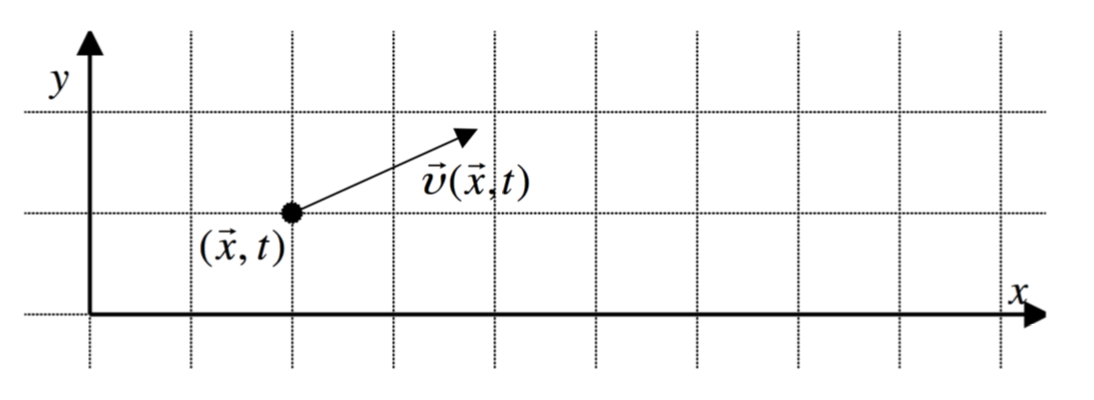
\includegraphics[scale = 0.4]{Figures/grid_method.png}
        \caption{Grid description, $retrieved from MIT(2011)$}
    \end{figure}

\section{Smoothed Particle Hydrodynamics}
    Smoothed particle hydrodynamics (SPH) was invented to simulate nonaxisymmetric phenoma in astrophysis initially. The principal idea of SPH is to treat hydrodynamics in a completely mesh-free fashion, in terms of a set of sampling particles. It turns out that the particle presentation of SPH has excellent conservation properties. Energy, linear momentum, angular momentum, mass and velocity.

    \subsection{Fundamentals}

    At the heart of SPH is a kernel interpolation method which allows any function to be expressed in terms of its values at a set of disordered points - the particles\cite{monaghan1992smoothed}. For ant field $A(\textbf{r})$, a smoothed interpolated version $A_{I}(\textbf{r})$ can be defined by a kernel $W(\textbf{r}, h)$,
    \begin{equation}
        A_{I}(\textbf{r}) = \int A({\textbf{r}}^{\prime})W(\|\textbf{r} - \textbf{r}^{\prime}\|, h)\dif\textbf{r}^{\prime}
    \end{equation}
    \begin{figure}[!ht]
        \centering
        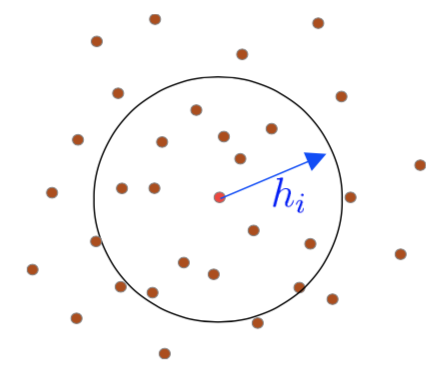
\includegraphics[scale = 0.6]{Figures/sph}
        \caption{Visilaztion of SPH}
    \end{figure}

    where the integration is over the entire space, and $W$ is an interpolating kernel with 
    \begin{equation}
        \int W(\|\textbf{r} - \textbf{r}^{\prime}\|, h)\dif \textbf{r}^{\prime} = 1
    \end{equation}
    and
    \begin{equation}
        \lim_{h\to 0} W(\|\textbf{r} - \textbf{r}^{\prime}\|, h)\dif\textbf{r}^{\prime} = \delta(\|\textbf{r} - \textbf{r}^{\prime}\|) 
    \end{equation}

    Normally, we want the kenel to be Non-negative and rotational invariant.
    \begin{equation}
        W(\|\textbf{x}_{i} - \text{x}_{j}\|, h) = W(\|\text{x}_{j} - \text{x}_{i}\|, h)
    \end{equation}

    \begin{equation}
        W(\|\textbf{r} - \textbf{r}^{\prime}\|, h) \ge 0
    \end{equation}

    For numerical work, we can use midpoint rule,
    \begin{equation}
        A_{I}(\textbf{x}) \approx A_{S}(\textbf{x}) = \sum_{i} A(\textbf{x}_{i})W(\|\textbf{x}_{i}-\textbf{x}\|, h)\Delta V_{i}
    \end{equation}
    Since $V_{i} = m_{i}/\rho _{i}$
    \begin{equation}
        A_{S}(\textbf{x}) = \sum_{i} \frac{m_{i}}{\rho_{i}} A(\textbf{x}_{i})W(\|\textbf{x}_{i}-\textbf{x}\|, h)
    \end{equation}

    The default, gradient and Laplacian of $A$ are:
    \begin{equation}
        \begin{aligned}
            \nabla A_{S}(\textbf{x}) &= \sum_{i} \frac{m_{i}}{\rho_{i}} A(\textbf{x}_{i})\nabla W(\|\textbf{x}_{i}-\textbf{x}\|, h) \\
            \nabla^{2} A_{S}(\textbf{x}) &= \sum_{i} \frac{m_{i}}{\rho_{i}} A(\textbf{x}_{i})\nabla^{2} W(\|\textbf{x}_{i}-\textbf{x}\|, h)
        \end{aligned}
        \label{eq:1}
    \end{equation}

    \subsection{Kernels}
    Smoothing kernels functions are one of the most important points in SPH. Stability, accurancy and speed of the whole method depends on these fuctions. Different kernels are being used for different purposes. One possibilyty for $W$ is a Gaussian. However, most current SPH implementations are based on kernels with finite support. We mainly introduce gaussian, poly6 and spicky kernel here. And compare the different kernels and their property.

    \subsubsection{Poly6}
    The kernel is also known as the 6th degree polynomial kernel.
    \begin{equation}
        W_{poly 6}(\textbf{r}, h) = \frac{315}{64\pi h^{9}}
            \begin{cases}
                (h^2 - \|\textbf{r}\|^2)^3 & 0 \le \|\textbf{r}\| \le h \\
                0 & \textrm{Otherwise}
            \end{cases}
    \end{equation}

    Then, the gradient of this kernel function can be
    \begin{equation}
        \nabla W_{poly 6}(\textbf{r}, h) = - \frac{945}{32\pi h^9}
            \begin{cases}
                \textbf{r}(h^2 - \|\textbf{r}\|^2)^2 & 0\le\|\textbf{r}\|\le h \\
                0 & \textrm{Otherwise}\\
            \end{cases}
    \end{equation}

    The laplacian of this kenel can be expressed by, 
    \begin{equation}
        \nabla^2 W_{poly6}(\textbf{r}, h) = - \frac{945}{16\pi h^9}
            \begin{cases}
                (h^2 - \|\textbf{r}\|^2)(3h^2-7\|\textbf{r}\|^2) & 0\le\|\textbf{r}\|\le h \\
                0 & \textrm{Otherwise}\\
            \end{cases}
    \end{equation}

    \subsubsection{Spicky}

    The kernel proposed by Desbrum\cite{desbrun1996smoothed}
    \begin{equation}
        W_{spiky}(\textbf{r}, h) = \frac{15}{\pi h^6}
            \begin{cases}
                (h - \|\textbf{r}\|)^3 & 0\le\|\textbf{r}\|\le h \\
                0 & \textrm{Otherwise}\\
            \end{cases}
    \end{equation}

    Then, the gradient of spiky kernel can be described by,
    \begin{equation}
        \nabla W_{spiky}(\textbf{r}, h) = -\frac{45 \textbf{r}}{\pi h^6 \|\textbf{r}\|}
            \begin{cases}
                (h - \|\textbf{r}\|)^2 & 0\le\|\textbf{r}\|\le h \\
                0 & \textrm{Otherwise}\\
            \end{cases}
    \end{equation}
     The laplacian of spiky can be expressed by,
     \begin{equation}
        \nabla^2 W_{spiky}(\textbf{r}, h) = \frac{90}{\pi h^6}
            \begin{cases}
                h - \| \textbf{r} \| & 0 \le \| \textbf{r} \| \le h \\
                0 & \textrm{Otherwise}\\
            \end{cases}
    \end{equation}

    \begin{figure}[!ht]
        \centering
        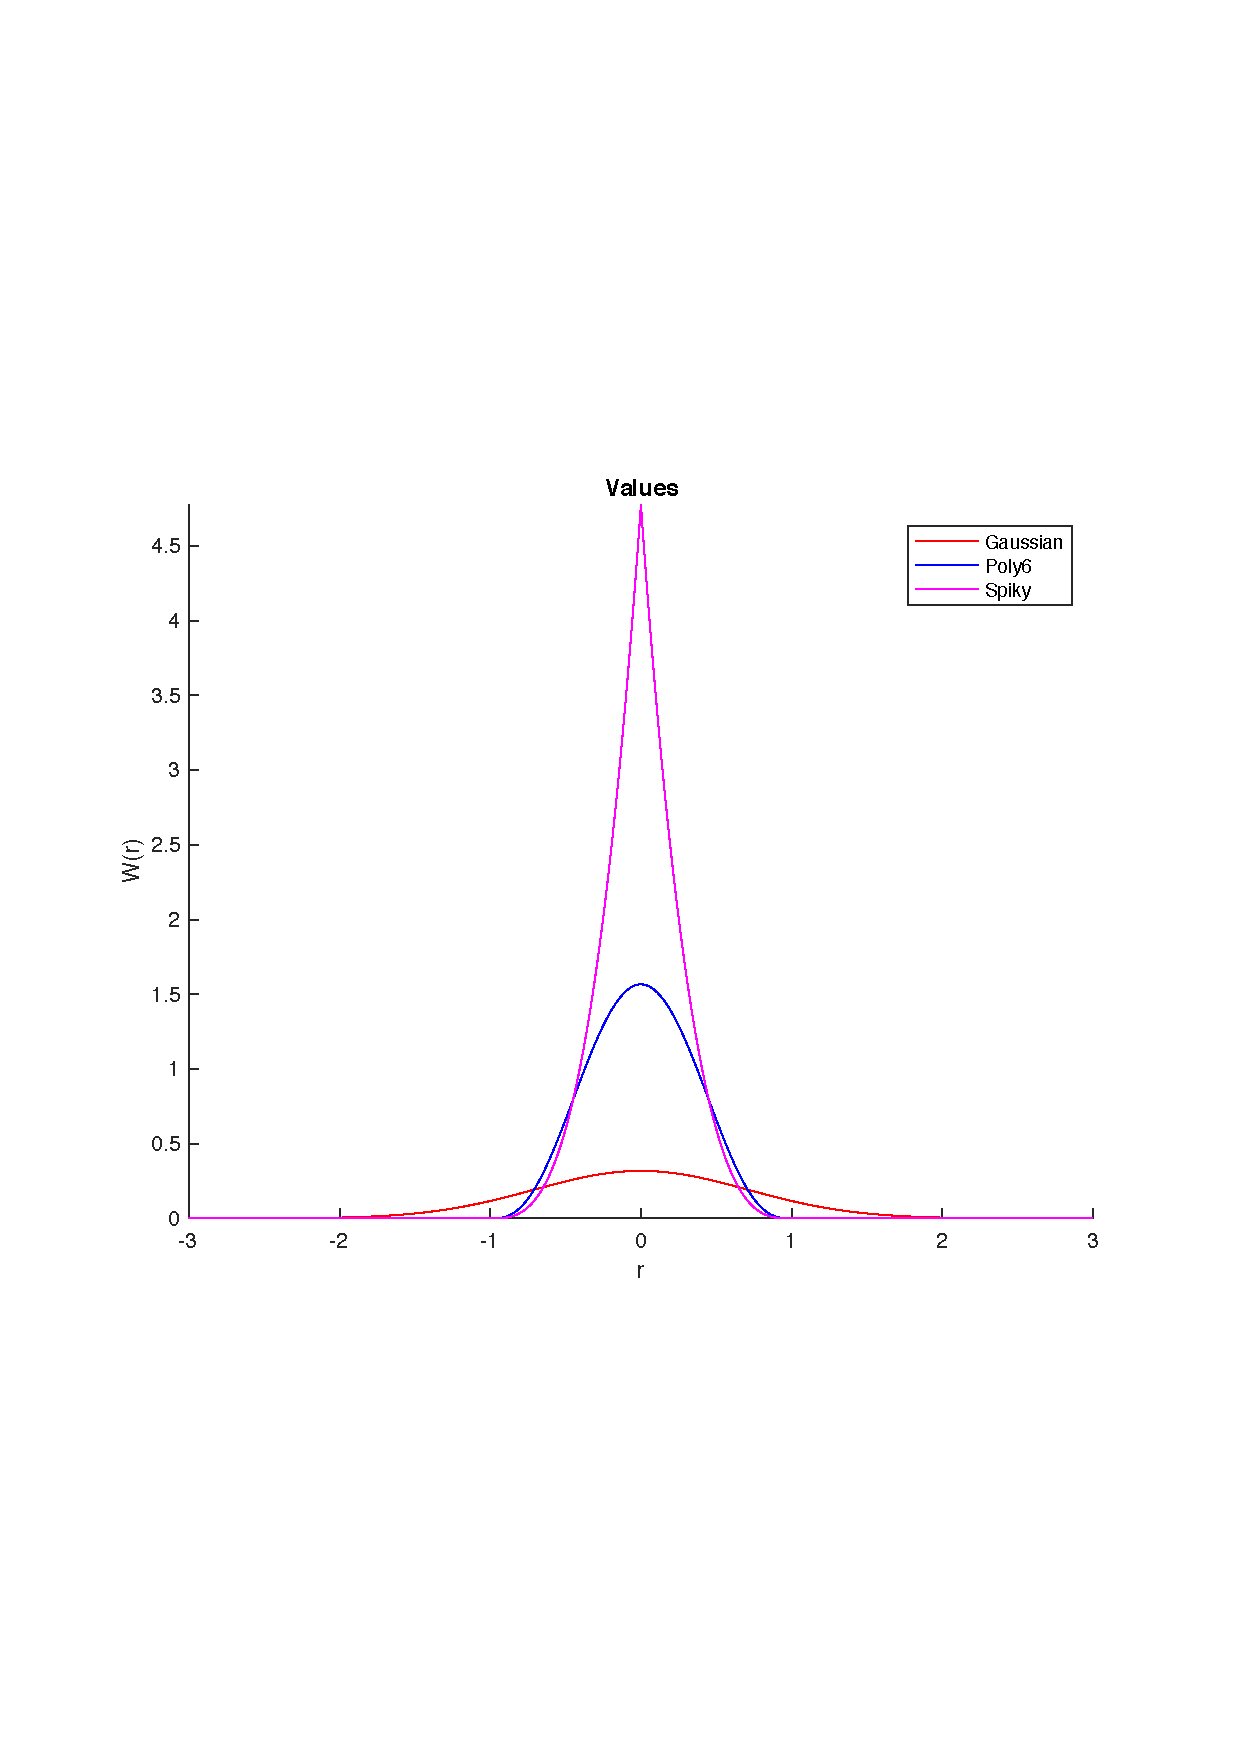
\includegraphics[scale = 0.5]{Figures/kernels}
        \caption{Comparation of different kernels, we set smoothing length $h = 1$ here.}
    \end{figure}

    \begin{figure}[!ht]
        \centering
        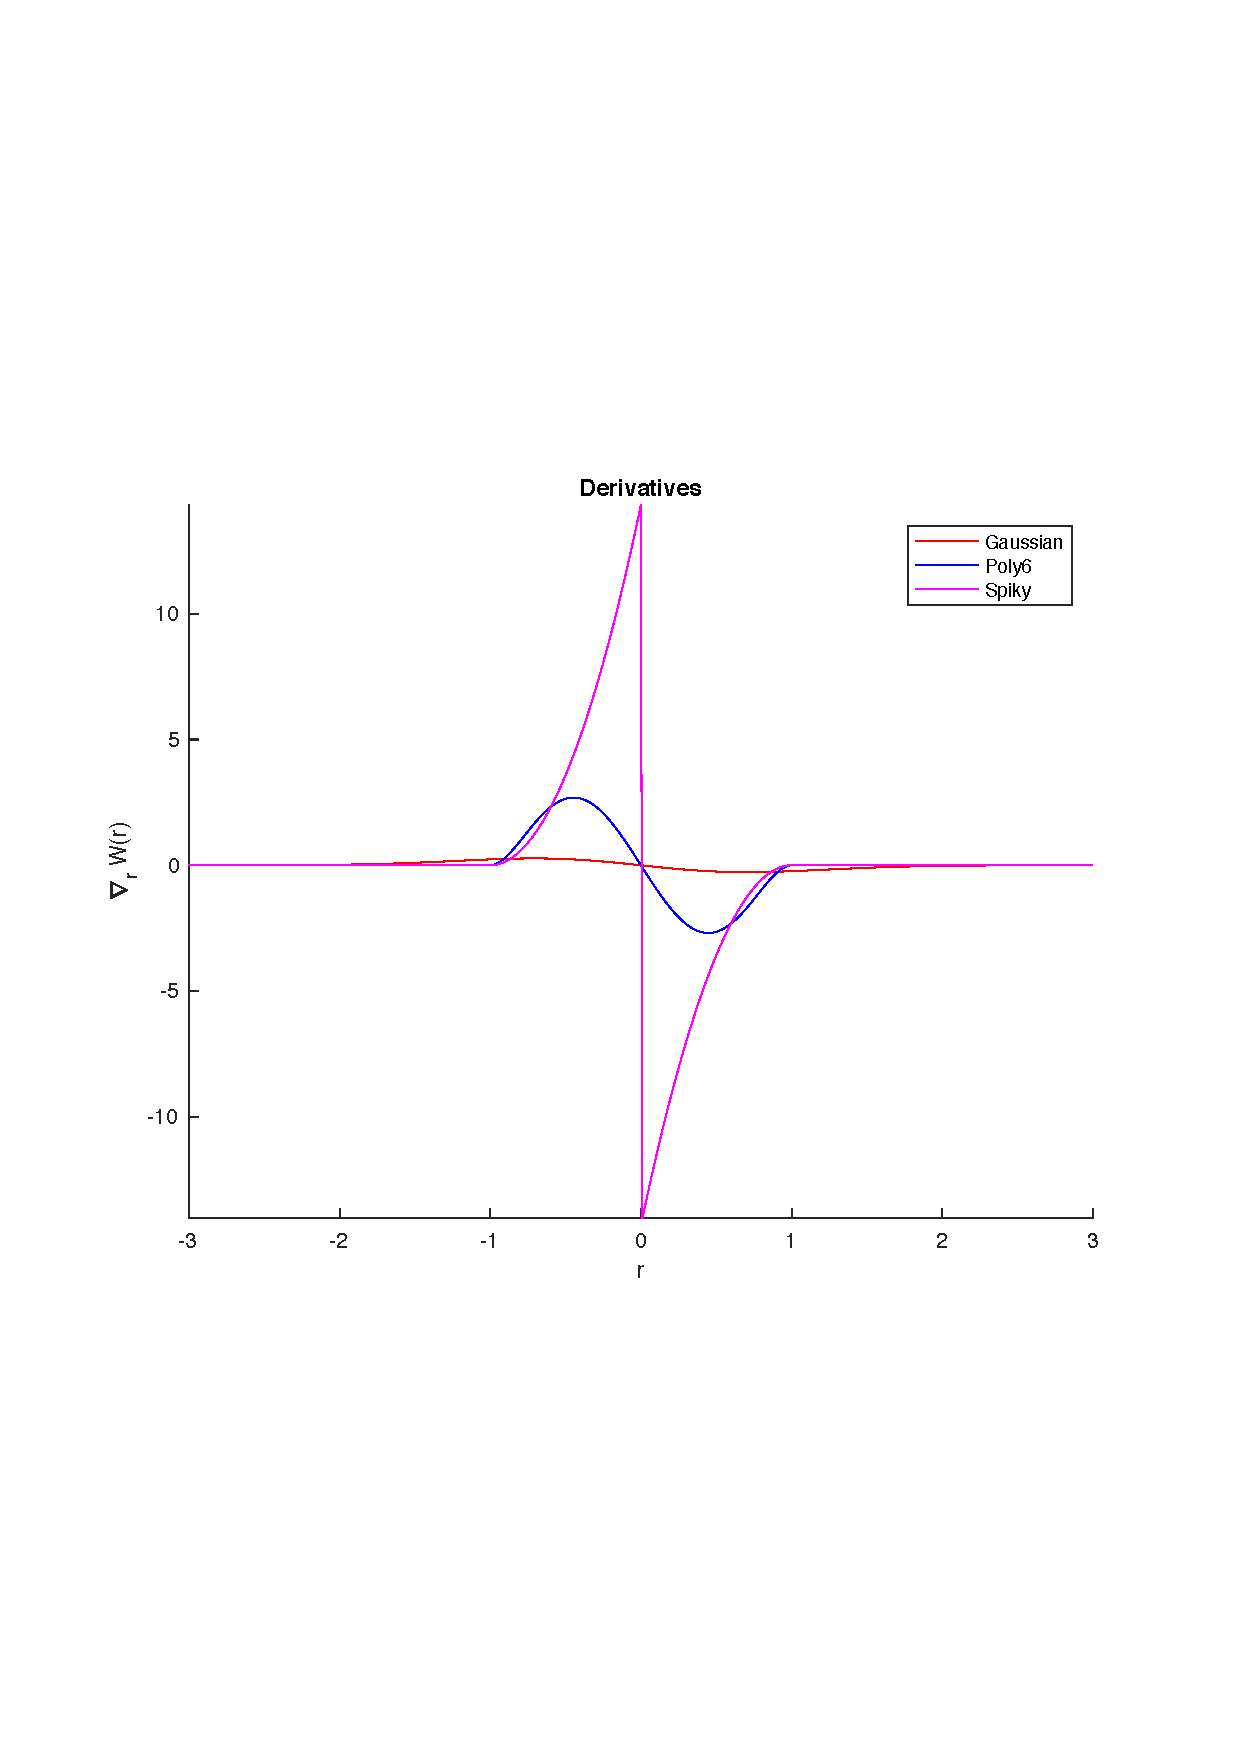
\includegraphics[scale = 0.5]{Figures/kenels_de}
        \caption{Comparation of gradient of different kernels, we set $h = 1$ here. }
    \end{figure}

    \subsection{Grid size and smoothing length}

    The grid should be also fine enough to capture the variation in our simulation. In our case, it is reasonable to have a grid fine enough such that no two contact points are mapped into the same cell. \\

    Smoothing length, $h$, is one of the most important parameters that affects the whole SPH method by changing the kernel value results abd neighbor searching results. Too small or too big values might cause lose essencail information in the simulation.

    \subsection{Neignbor Search}
    Neighbor search is one of the most crucial procedures in SPH method considersing all interpolation equations, $A(\textbf{r})$, needs the neighbor list for every particle (refer to equation \ref{eq:1}). A naive neighbor searching approach would end up with a complexity of $o(n^2)$. The complexity is not good enough since it is impossoble to reach any interactive speed when the particle count increses. With an efficient nearest neighbor searching(NNS) algorithm, it is possible to have a significant performance increase since it is the most time consuming procedure in SPH computation. In order to decrease the complexity, we choose to use $k-d$ tree data structure to store the particla spatial information and then do the nearest neighbor searching.

        \subsubsection{Hierarchical Tree}
        Using an adaptive hierarchy tree search is proposed by Paiva\cite{paiva2006particle} to find particle neighbors. Since the simulation takes place in two dimensions, $k-d$ tree data structure was used in this approach. \\

        An octree structure has been adapted from Macey (b) Octree Demo. The hierarchy tree is formed with a pre-defined height. The simulation box is divided recursively into eight pieces, nodes. The nodes at height = 1 are called leaves. Each node has a surrounding box for particle query which is used to check if the particle is inside the node. Each parent node, contains the elements that are divided through its children. The particle is being checked at each level of the tree if it’s intersecting the node. If it does, descend one level down in that node. After reaching to leaves, bottom level, particle has been checked if its within the search distance, $h$. If the particle is in the range, add it to the neighbor list. Neighbor searching is done when the whole tree has been traversed. The search distance set to be smoothing length in this implementation. \\

        The complexity of this tree search method is $O(nlog(n))$, n being the number of particles. The performance of this algorithm is worse than Spatial Hashing method. In addition, the results obtained using this NNS algorithm wasn’t accurate and stable for this implementation. Therefore as mentioned above, Spatial Hashing method was preferred.


\section{Grid to particle}
    After getting the grid image for simulation state in time $t$, we will use the grid cells as input and renew the grid image based on trained model. Once the grid image in $t+\Delta t$ have been renewed, the next step is to transfer the grid to particles which will instore all information including velocity,  
    \subsection{Bilinear interpolation}
    We applied bilinear interpolation in our case, since we did mainly research on a rectilinear $2-D$ grid.
    \begin{figure}[!ht]
        \centering
        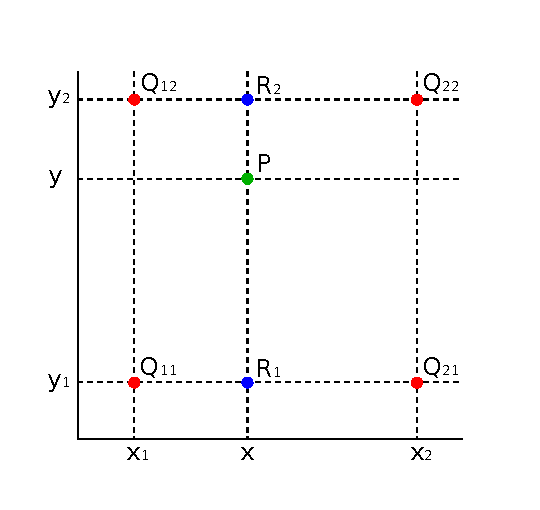
\includegraphics[scale = 0.5]{Figures/inp}
        \caption{The figure shows visiualization of bilinear interpolation. The four red dots show the data points and the green dot is the point at which we want to interpolate.}
        \label{fig:1}
    \end{figure}
    The key idea is to perform linear interpolation first in one direction, and then again in the other direction. Although each step is linear in the sampled values and in the position, the interpolation as a whole is not linear but rather quadratic in the sample location. \\

    As shown in Figure \ref{fig:1}, We have known $Q_{a, b} = (x_a, y_ b)$. Then, we can firstly do linear interpolation in the $x$-direction. This yields

    \begin{equation}
        \begin{aligned}
            f(x,y_{1})&\approx {\frac {x_{2}-x}{x_{2}-x_{1}}}f(Q_{11})+{\frac {x-x_{1}}{x_{2}-x_{1}}}f(Q_{21}),\\f(x,y_{2})&\approx {\frac {x_{2}-x}{x_{2}-x_{1}}}f(Q_{12})+{\frac {x-x_{1}}{x_{2}-x_{1}}}f(Q_{22}).
        \end{aligned}
        \label{eq:2}
    \end{equation}

    After getting the two values in $x-$direction $f(x, y_1)$ and $f(x, y_2)$, we can use these values to do interpolation in $y-$ direction.
    \begin{equation}
        f(x,y) \approx {\frac {y_{2}-y}{y_{2}-y_{1}}}f(x,y_{1})+{\frac {y-y_{1}}{y_{2}-y_{1}}}f(x,y_{2})
    \end{equation}

    Combine $f(x, y_1)$ and $f(x, y_2)$ defined in equation \ref{eq:2}, we can get,

    \begin{equation}
        \begin{aligned}
        f(x,y)&\approx{\frac {y_{2}-y}{y_{2}-y_{1}}}\left({\frac {x_{2}-x}{x_{2}-x_{1}}}f(Q_{11})+{\frac {x-x_{1}}{x_{2}-x_{1}}}f(Q_{21})\right)\\&\qquad+{\frac {y-y_{1}}{y_{2}-y_{1}}}\left({\frac {x_{2}-x}{x_{2}-x_{1}}}f(Q_{12})+{\frac {x-x_{1}}{x_{2}-x_{1}}}f(Q_{22})\right)\\&={\frac {1}{(x_{2}-x_{1})(y_{2}-y_{1})}}{\big (}\\&\qquad f(Q_{11})(x_{2}-x)(y_{2}-y)+f(Q_{21})(x-x_{1})(y_{2}-y)\\&\qquad+f(Q_{12})(x_{2}-x)(y-y_{1})+f(Q_{22})(x-x_{1})(y-y_{1}){\big )}\\&={\frac {1}{(x_{2}-x_{1})(y_{2}-y_{1})}}{\begin{bmatrix}x_{2}-x&x-x_{1}\end{bmatrix}}\\&\qquad \cdot {\begin{bmatrix}f(Q_{11})&f(Q_{12})\\f(Q_{21})&f(Q_{22})\end{bmatrix}}{\begin{bmatrix}y_{2}-y\\y-y_{1}\end{bmatrix}}
        \end{aligned}
    \end{equation}

\section{Conclution}
    \chapter{Deep Learning For Simulation}


\section{Convolutional Neural Networks}

\section{CNN Constructure}
    \subsection{Convolutional layers}

    \subsection{Full-connected layers}

\section{Traing configuration}
    \subsection{Loss Function}

    \subsection{Optimizer(SGD)}

\section{Training Results}

\section{Simulation based on Trained model}
    \chapter{Results and Analysis}
\label{details}
After introducing the basic knowledge which is available and used in the project, I will start the experiments and analyze the results. The main experiments would be,
\begin{enumerate}
    \item Do the simulation based one computer physics library(\textit{pybox2d}). Totally, 100 different rigid motion simulation would be carried out. For every simulation, I would record the fixed number of simulation steps, $600$.
    \item \textbf{XML} formulation would be used to store every step of all simulation. The data of each state would involve positions, velocities, contact forces, etc.
    \item Once obtaining the \textbf{XML} files. I would transform the \textbf{XML} files into a \textit{pybox2d} world, and then carry out some experiments to determine different grid size and smoothing length of SPH.
    \item After choosing the proper parameter of the SPH kernel(types, grid cell size, and smoothing length), I would transform these \textbf{XML} files to grid images, which are used as training dataset. 
    \item Design a deep learning model and do the training on the training dataset.
    \item Apply the trained model to predict the starting iterate values of contact forces($\pmb{\lambda}$). Then I would compare the learning model with other classical methods.
\end{enumerate}

\section{Rigid Motion Simulation}

\textit{pybox2d}\footnote{\url{https://github.com/pybox2d/pybox2d}} is chosen as the main physics engine to implement computer simulation experiments. \textit{pybox2d} is a 2D physics library for your games and simple simulations. It's based on the Box2D library, which is written in \textit{C++}. It supports several shape types (circle, polygon, thin line segments), and quite a few joint types (revolute, prismatic, wheel, etc.). In my experiment, I would first try to apply deep learning in the simple simulations. So I would mainly simulation with circle rigid objects sharing the same radius. 

\subsection{Simulation Configuration}
Simulation configs are listed below,
    \label{simconfig}
    \begin{itemize}
        \item \textbf{World Setting}, the world box size is $30\times30$,   and there are $100$ circle rigids($r=1$, all circle rigid bodies in the same size.) inside the box. Initially, the rigid circles will be located following gaussian distribution\footnote{\url{https://en.wikipedia.org/wiki/Normal_distribution}}. Then, all rigid circles will fall down by gravity. The visualization of simulation is shown in Figure \ref{fig:imsim}.
        \item \textbf{Simulation Setting}, there will be totally $600$-steps simulation. For each step, $\Delta t = 0.01s$, and the number of iteration in each step will be set as fixed, $3000$. Then I will use the average convergence rate to describe the performances of models.
    \end{itemize}
\subsection{Simulation Details}
    Before generating data, one dynamic simulation was run to check how \textit{pybox2d} works and some figures have been obtained. Figure \ref{fig:contactnum} describe the relationship between time step and contacts number, and Figure \ref{fig:contacttime} gives the relationship between time spend and contacts number.
    \begin{figure}[!h]
        \centering
        \begin{subfigure}[b]{0.3\textwidth}
            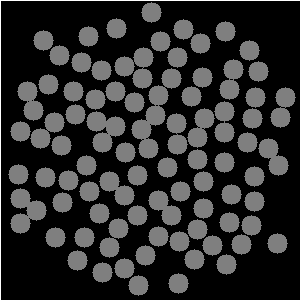
\includegraphics[width=\textwidth]{Figures/sim0.png}
            \caption{Time Step=$0$}
        \end{subfigure}
        \begin{subfigure}[b]{0.3\textwidth}
            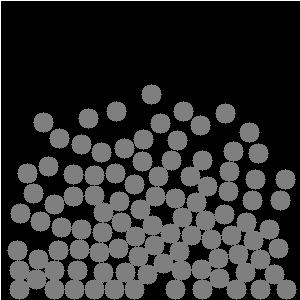
\includegraphics[width=\textwidth]{Figures/sim2.png}
            \caption{Time Step=$200$}
        \end{subfigure}
        \begin{subfigure}[b]{0.3\textwidth}
            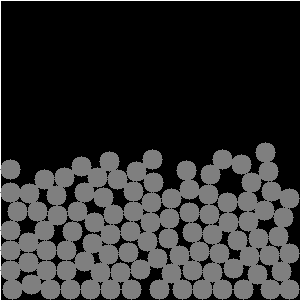
\includegraphics[width=\textwidth]{Figures/sim3.png}
            \caption{Time Step=$400$}
        \end{subfigure}
        \caption{Visualization for experiment simulation}
        \label{fig:imsim}
    \end{figure}
    \begin{figure}[!ht]
        \centering
        \begin{subfigure}[b]{0.7\textwidth}
            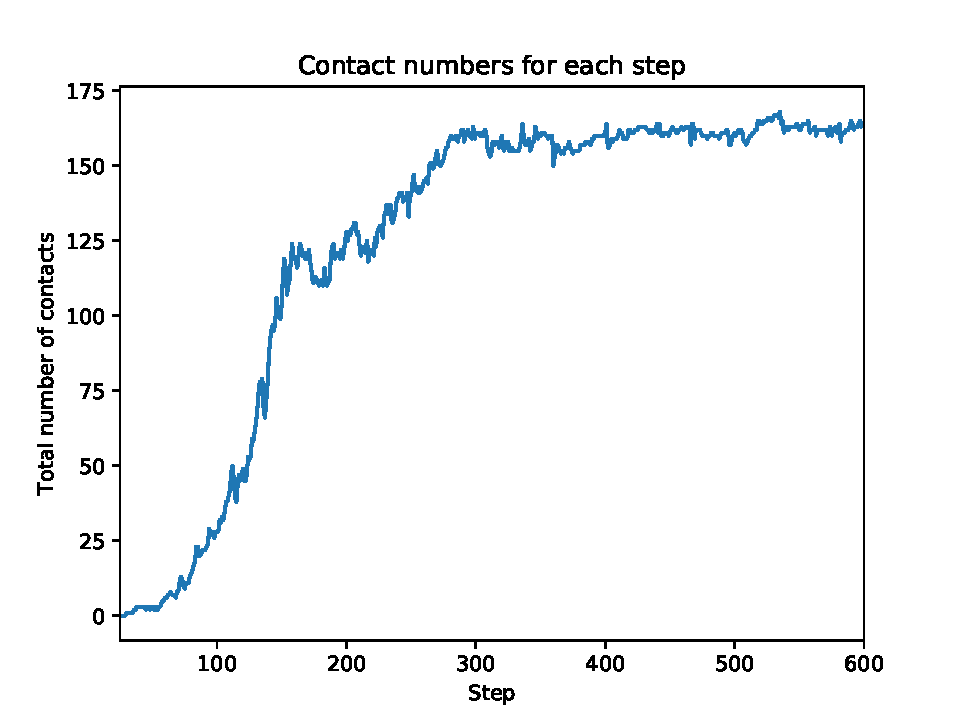
\includegraphics[width=\textwidth]{Figures/contact_num}
            \caption{The number of contacts in each step.}
            \label{fig:contactnum}
        \end{subfigure}
        \begin{subfigure}[b]{0.7\textwidth}
            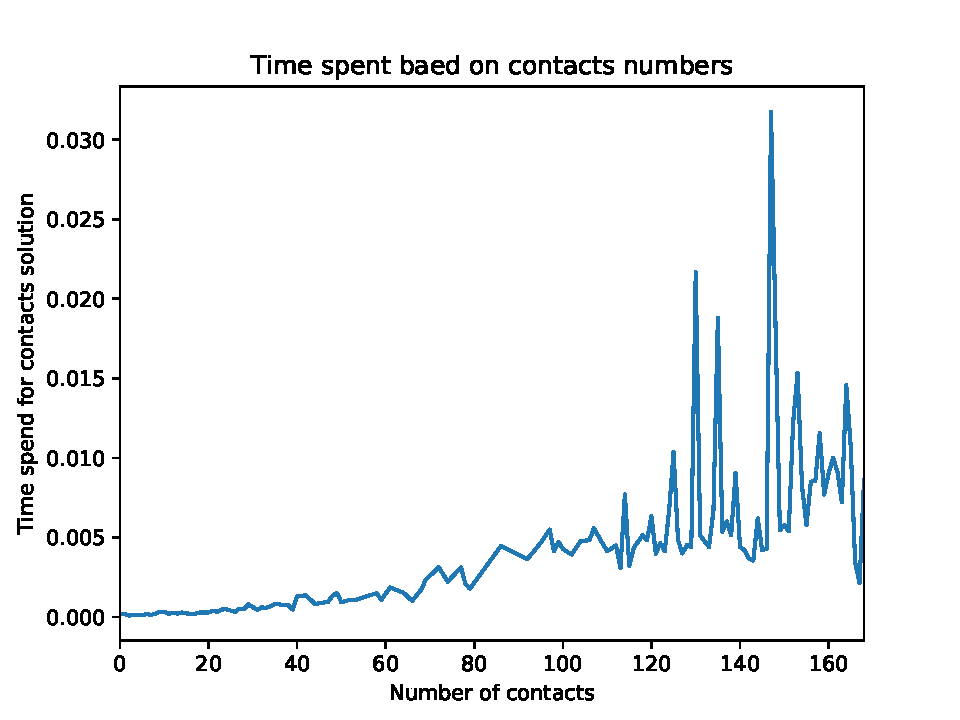
\includegraphics[width=\textwidth]{Figures/contact_time}
            \caption{Time spent for contact solutions.}
            \label{fig:contacttime}
        \end{subfigure}
        \caption{Visualization for experiment simulation}
    \end{figure}

\subsection{SPH parameters}
    \label{SPH-setting}
    In Section \ref{sphtest}, it has been tested that \textbf{SPH} is a good strategy to generate grid images representing a discrete snapshot of the dynamics. Then, the grid size and smoothing length $h$ are imported into our data generation. The grid size should be reasonable so that there is no two contact points are mapped into the same cell, since if there are more than two contact values in one cell, the rid node might store mixture information state from two objects. which would be hard for CNN to find the relationship within one objects, which will decrease the accuracy of prediction. This was mentioned in section \ref{gs}.
    \begin{figure}[!h]
        \centering
        \includegraphics[width=0.4\textwidth]{Figures/SPHvi.pdf}
        \caption{Example visiualization for Smoothed Particle Hydrodynamics. The small red circles stand for the grid nodes, and the blue circles stand for kernel size.}
    \end{figure}

    \subsubsection{Grid Size and Kernel Length}
    I define $\pmb{d}=(d_x, d_y)$ as grid cell size and $h$ as smoothing length. I conclude some rules for determining grid cell size and smoothing length. 
    \begin{itemize}
        \item Since the objects are circles, the ideal cell size should like,
            $$d_x = d_y = d $$ 
        \item Since there can not be two contact points are mapped into the same cell, $d$ must be less than the distance of nearest two contact points. It can be defined.
            $$d \le r = 1$$
        \item Similarly, if one contact point can only be mapped to one cell, the smooth length $h$ should be less than the minimum distance between two contact points $d$,
            $$h \le d$$  
        \item For a given $d$, whatever the contact position $\pmb{q}=(q_x, q_y)$ is, its information can be restore in nearby nodes. So it can be,
            $$h \ge \frac{\sqrt{2}}{2}d \approx 0.71 d$$
    \end{itemize}
    One experiment has been designed to test whether the rules can be applied in this case. Still using the simulation config introduced in section \ref{simconfig}. The cell size is fixed, $d=0.25$. Different smoothing length is appiled. The results are shown in Figure \ref{fig:dh}.

    \begin{figure}[!ht]
     \centering
    \begin{subfigure}[b]{0.7\textwidth}
        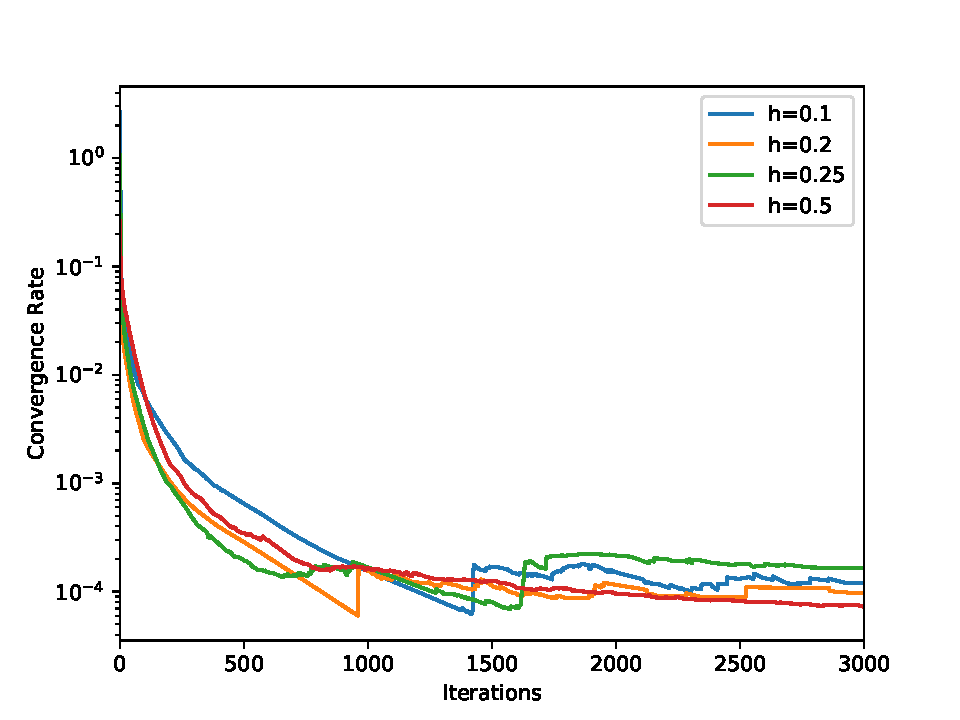
\includegraphics[width=\textwidth]{Figures/size25.pdf}
        \caption{The grid size $d$ is set $0.25$. $h=0.1, 0.2, 0.25, 0.5$ is tested respectively. This figure shows different coveragence rate based on different $h$ value.}
        \label{fig:dh}
    \end{subfigure}
    \begin{subfigure}[b]{0.7\textwidth}
        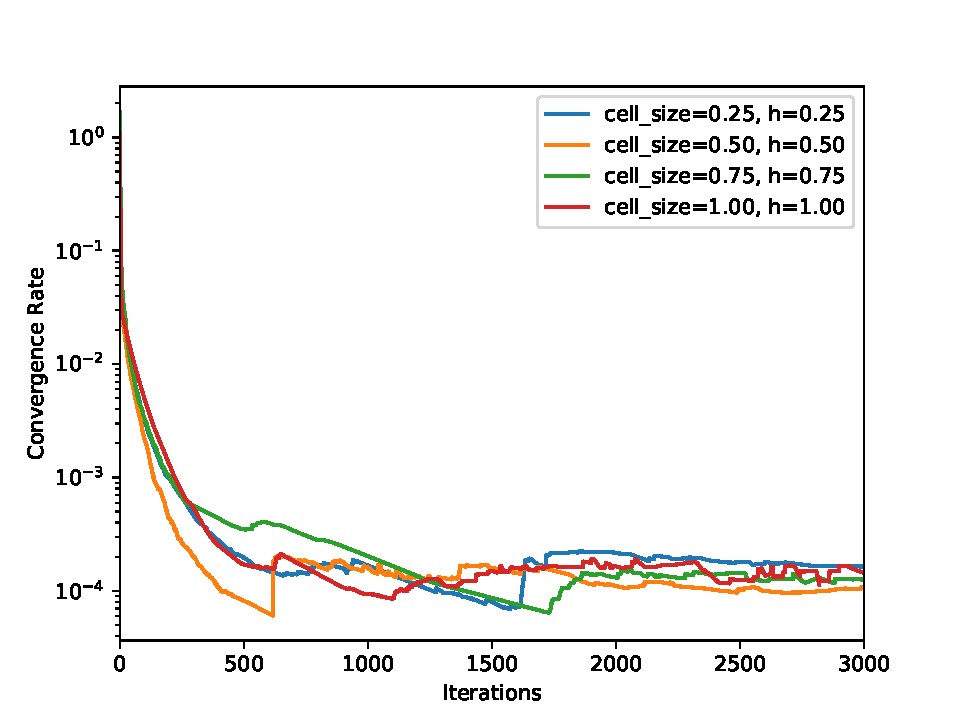
\includegraphics[width=\textwidth]{Figures/hd.pdf}
        \caption{Coveragence rate for different $d$ value.}
        \label{fig:testd}
    \end{subfigure}
    \caption{Experiments from kernel \textbf{Poly6}}
    \label{poly6}
    \end{figure}

    As what is shown in Figure \ref{fig:dh}, when $h=0.4d$ or $h=2d$, the solver coverages more slowly and unstable. Overall, for the next step, data generation, I will make $h=d$ always. The next step is to explore what $d$ value will be good. Once $h=d$ has been determined, the next step is to choose the value of $d$. Another experiment is taken to check the convergence rate with using diffrent $d$ values. The reults are showns in Figure \ref{fig:testd}. From this figure, it is obviously, when $d=0.5$, iterative solver converages the most rapidly. 
    \textbf{Importantly}, $d=0.5~~\text{and}~~h=0.5$ is not always the best experimented with different numbers of rigid inside the world box. But, it generally performs better than other values. As a result, I will choose $h=d=0.5$ as the parameters for SPH method.
    $$d_x = d_y = 0.5~~\text{and}~~h=0.5$$
    \subsubsection{Kernel Choosing}
    The choice of kernel also needs to be addressed. In the paper, two kernels, \textbf{Poly6} and \textbf{Spiky}, have been introduced in section \ref{sec:kernels}. In order to compare these two kernels and determine the best one, finding the best parameters for \textbf{Spiky} is essential. I did the same experiment with kernel \textbf{Spiky}. Find a good scale between $h$ and $d$ firstly and then choose $d$. The results are shown in Figure \ref{spiky}. The plot in Figure \ref{fig:spikynum} reveals that $h=d$ is also a good choice for kernel \textbf{Spiky}. Although $d$s perform similarly, $d=0.25$ performs more stable and a bit fater in convergence. \\
    \begin{figure}[!ht]
        \centering
        \begin{subfigure}[b]{0.7\textwidth}
            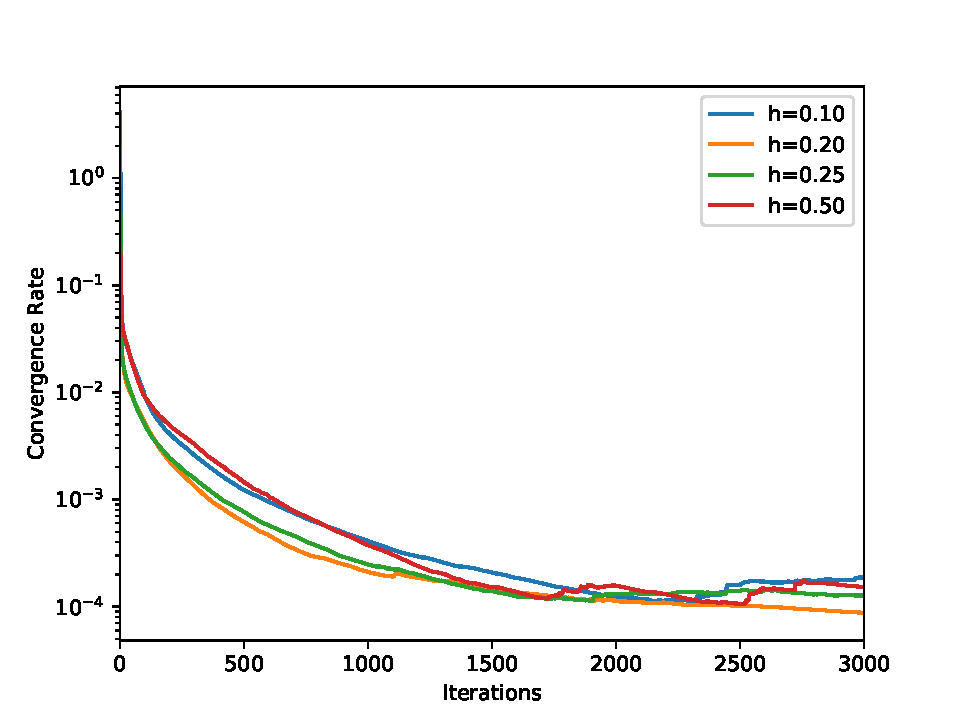
\includegraphics[width=\textwidth]{Figures/spiky25.pdf}
            \caption{The grid size $d$ is set $0.25$. $h=0.1, 0.2, 0.25, 0.5$ is tested respectively. This figure shows different coveragence rate based on different $h$ value.}
            \label{fig:spikynum}
        \end{subfigure}
        \begin{subfigure}[b]{0.7\textwidth}
            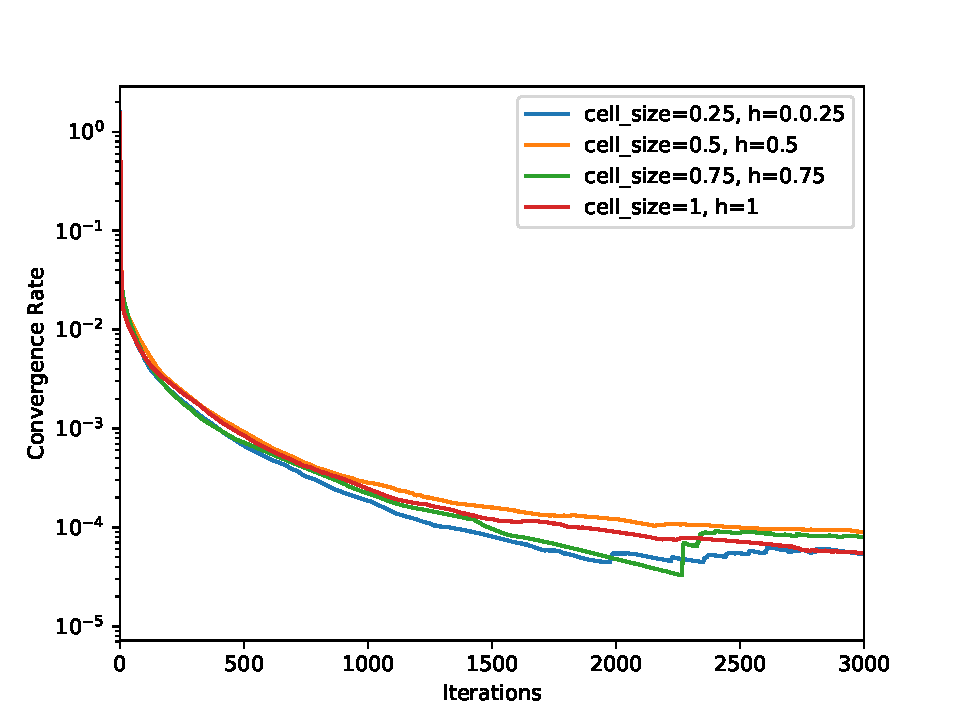
\includegraphics[width=\textwidth]{Figures/spikysize.pdf}
            \caption{Coveragence rate for different $d$ value.}
            \label{fig:spikyttime}
        \end{subfigure}
        \caption{Experiments for kernel \textbf{Spiky}.}
        \label{spiky}
    \end{figure}
    These two kernels are separately used based on Algorithm \ref{testsph}. In order to compare these two kernels carefully, the fixed iteration number was extended to $5000$. Then, the plot about the convergence rate of different kernels is obtained in Figure \ref{fig:testdkernel}. From the plot, it is clear that kernel \textbf{Poly6} perform better.  
    \begin{figure}[!ht]{}
        \centering
        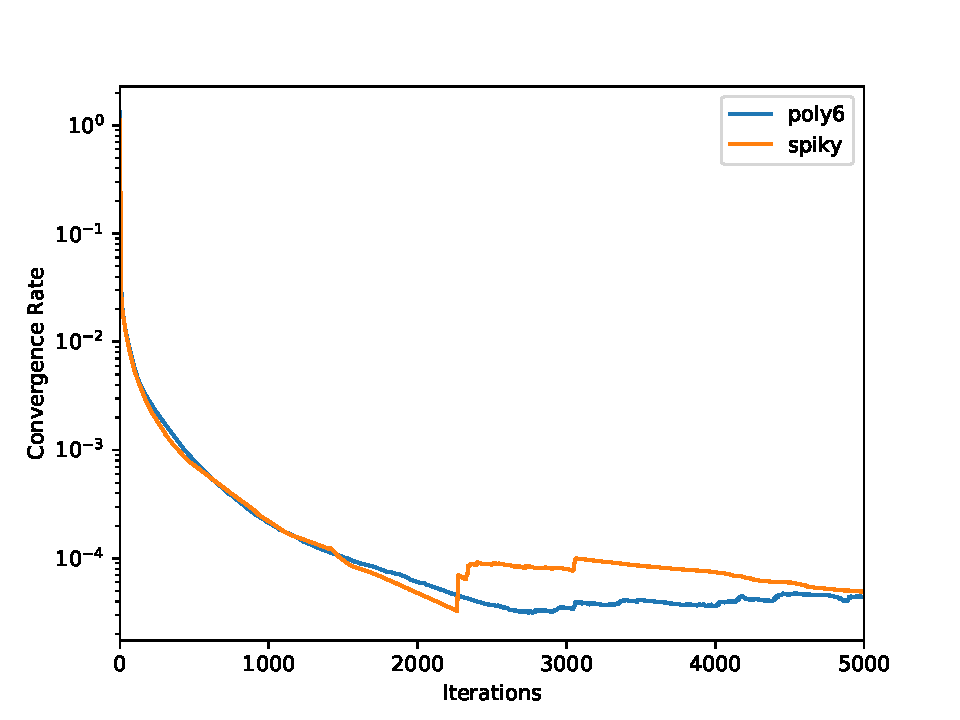
\includegraphics[width=0.8\textwidth]{Figures/kerneltest.pdf}
        \caption{Coveragence rate for kernel \textbf{Poly6} anf \textbf{Spiky}. $h_\text{poly6} = d_\text{poly6} = 0.5$, while $h_\text{spiky} = d_\text{spiky} = 0.25$}
        \label{fig:testdkernel}
    \end{figure}
    As a conclusion, SPH with \textbf{Poly6} kernel($\pmb{d} = (0.5, 0.5)$, smoothing length $h=0.5$), will be used for particle-grid transformation. \\

    After determining grid size and smoothing length, I will compare this specific \textbf{SPH-Model} with other models mentionde in section \ref{sphtest}, following Algorithm \ref{testsph}. The result is shown in Figure \ref{fig:final_test}.
     \begin{figure}[!ht]
        \centering
        \includegraphics[width=0.8\textwidth]{Figures/final_SPH.pdf}
        \caption{Coveragence rate for models(different initial values for $\pmb{\lambda}$).}
        \label{fig:final_test}
    \end{figure}
    Unlike the result shown in Figure \ref{fg:addsph}. Compared with other models, \textbf{SPH-Model} gets convergence much faster. So, $h=d=0.5$ is a good choice for this project and the future steps.

\section{Data Generation}
To create data that are more accessible to learning, I will map a discrete element method into a continuum setting use techniques from smooth particle hydrodynamics(SPH). In order to get enough available training data and remove useless information, I used,
\begin{itemize}
    \item Totally $150$ simulations with different initial configuration. The number of circle objects is not fixed as well. However, if there are too few objects inside the box, contacts might not happen until the simulation ends up. So the number of objects will be in the range of $[70, 110]$.
    \item If there is no contact in one state, the state means nothing to the learning. So the state files without any contacts will be removed.
\end{itemize}

\subsection{XML Restoration}
For each simulation, the state in every time step will be stored in one \textbf{XML} file. The structure of the body is consist of \textbf{mass}, \textbf{position}, \textbf{velocity}, \textbf{spin omega} and \textbf{inertia}. The structure of contact consists of \textbf{postion}, \textbf{impulse}(including in normal direction and tangent direcrion), \textbf{master} body and \textbf{slave} body. Two examples are given in the following.\\

This is an example of one body information is given below.
\begin{lstlisting}[language=XML]
    <body index="86" type="free">
        <mass value="3.14159274101"/>
        <position x="7.79289388657" y="2.62924313545"/>
        <velocity x="2.7878344059" y="-1.45545887947"/>
        <orientation theta="-0.115291565657"/>
        <inertia value="1.57079637051"/>
        <spin omega="-2.33787894249"/>
        <shape value="circle"/>
    </body>
    ...
\end{lstlisting}
Another example \textit{XML} code is for contatc force.
\begin{lstlisting}[language=XML]
    <contact index="1" master="2" master_shape="b2CircleShape(childCount=1, pos=b2Vec2(0,0), radius=1.2000000476837158, type=0,)" slave="97" slave_shape="b2CircleShape(childCount=1, pos=b2Vec2(0,0), radius=1.2000000476837158, type=0, )">
        <position x="0.21963849663734436" y="13.875240325927734"/>
        <normal normal="b2Vec2(-1,2.9819e-05)"/>
        <impulse n="0.005236322991549969" t="-0.002184529323130846"/>
    </contact>
    ...
\end{lstlisting}

\subsection{SPH configuration}
As it is talked in \ref{SPH-setting}, 
\begin{itemize}
    \item \textbf{Kernel}, Poly6, which you can see in section \ref{poly6}.
    \item \textbf{Kernel Settings}, cell size $d_x=d_y=0.5$, smoothing length $h=0.5$.
\end{itemize}
\subsection{XML to grid}
After getting a set of \textbf{XML} file, the next step is to load state information from \textbf{XML} file, and then map them to grid images with SPH based method. Since for any contact point, there are two normal contacts, one with $[n_x, n_y]$ while the other with $[-n_x, -n_y]$. So the grid values for $\pmb{n}$ would be always $\pmb{0}$, and the same  with $\pmb{t}$. So finally, the channel number of each image will be $6$, including $[m, v_x, v_y, \omega, \lambda_n, \lambda_t]$. \\

For the learning, I divide 8 channels into features(input) and label(output).
    $$\text{Feature} = [m, v_x, v_y, \omega]$$
    $$\text{Label} = [\lambda_n, \lambda_t]$$


\section{CNN Training}
\subsection{CNN  Architecture}
    The neural network was designed using Keras\cite{chollet2015keras}. Keras is a neural networks Application Programming Interface (API) written in Python, it runs on top of either TensorFlow. With some inspiration from AlexNet\cite{Krizhevsky:2012:ICD:2999134.2999257}, the networks shows five constructing stacks of layers and each stack is consist of two or three convolutional layers in the same size. To avoid overfitting, each stack is followed by one dropout layer. One full-connected layer is set after the last convolutional layer. This input layer is followed by a batch normalization layer, normalizing images within a batch, which is discussed in Section \ref{batchnor}. This architecture includes $51,599,092$ weights for an input size of ($61\times61\times4$). All convolutional layers have kernels of size $(3\times 3\times d)$, and are followed by ReLU activation function. Figure \ref{fig:art} shows the visualization of model architecture, and Table \ref{table:layers} shows the specific information about parameters when input images go through the CNN.
    \begin{itemize}
        \item \textbf{Input Size}, the input will be $61\times61\times4$. Since the orginal world is $30\times30$ and grid size is $d=0.5$, the generated grid would be $61\times61$. There would $4$ channels
        \item \textbf{Output Size}, output size depends on the label size. The orginal label image would be $[\lambda_n, \lambda_t]$, so the label image size would be $61\times61\times2$, which should be flattened as the actual training label. The label size would be $61\times 61 \times 2$
        \item \textbf{Weight Number}, the total weights number is $64,498,866$. 
    \end{itemize}

    \begin{figure}[!h]
        \centering
        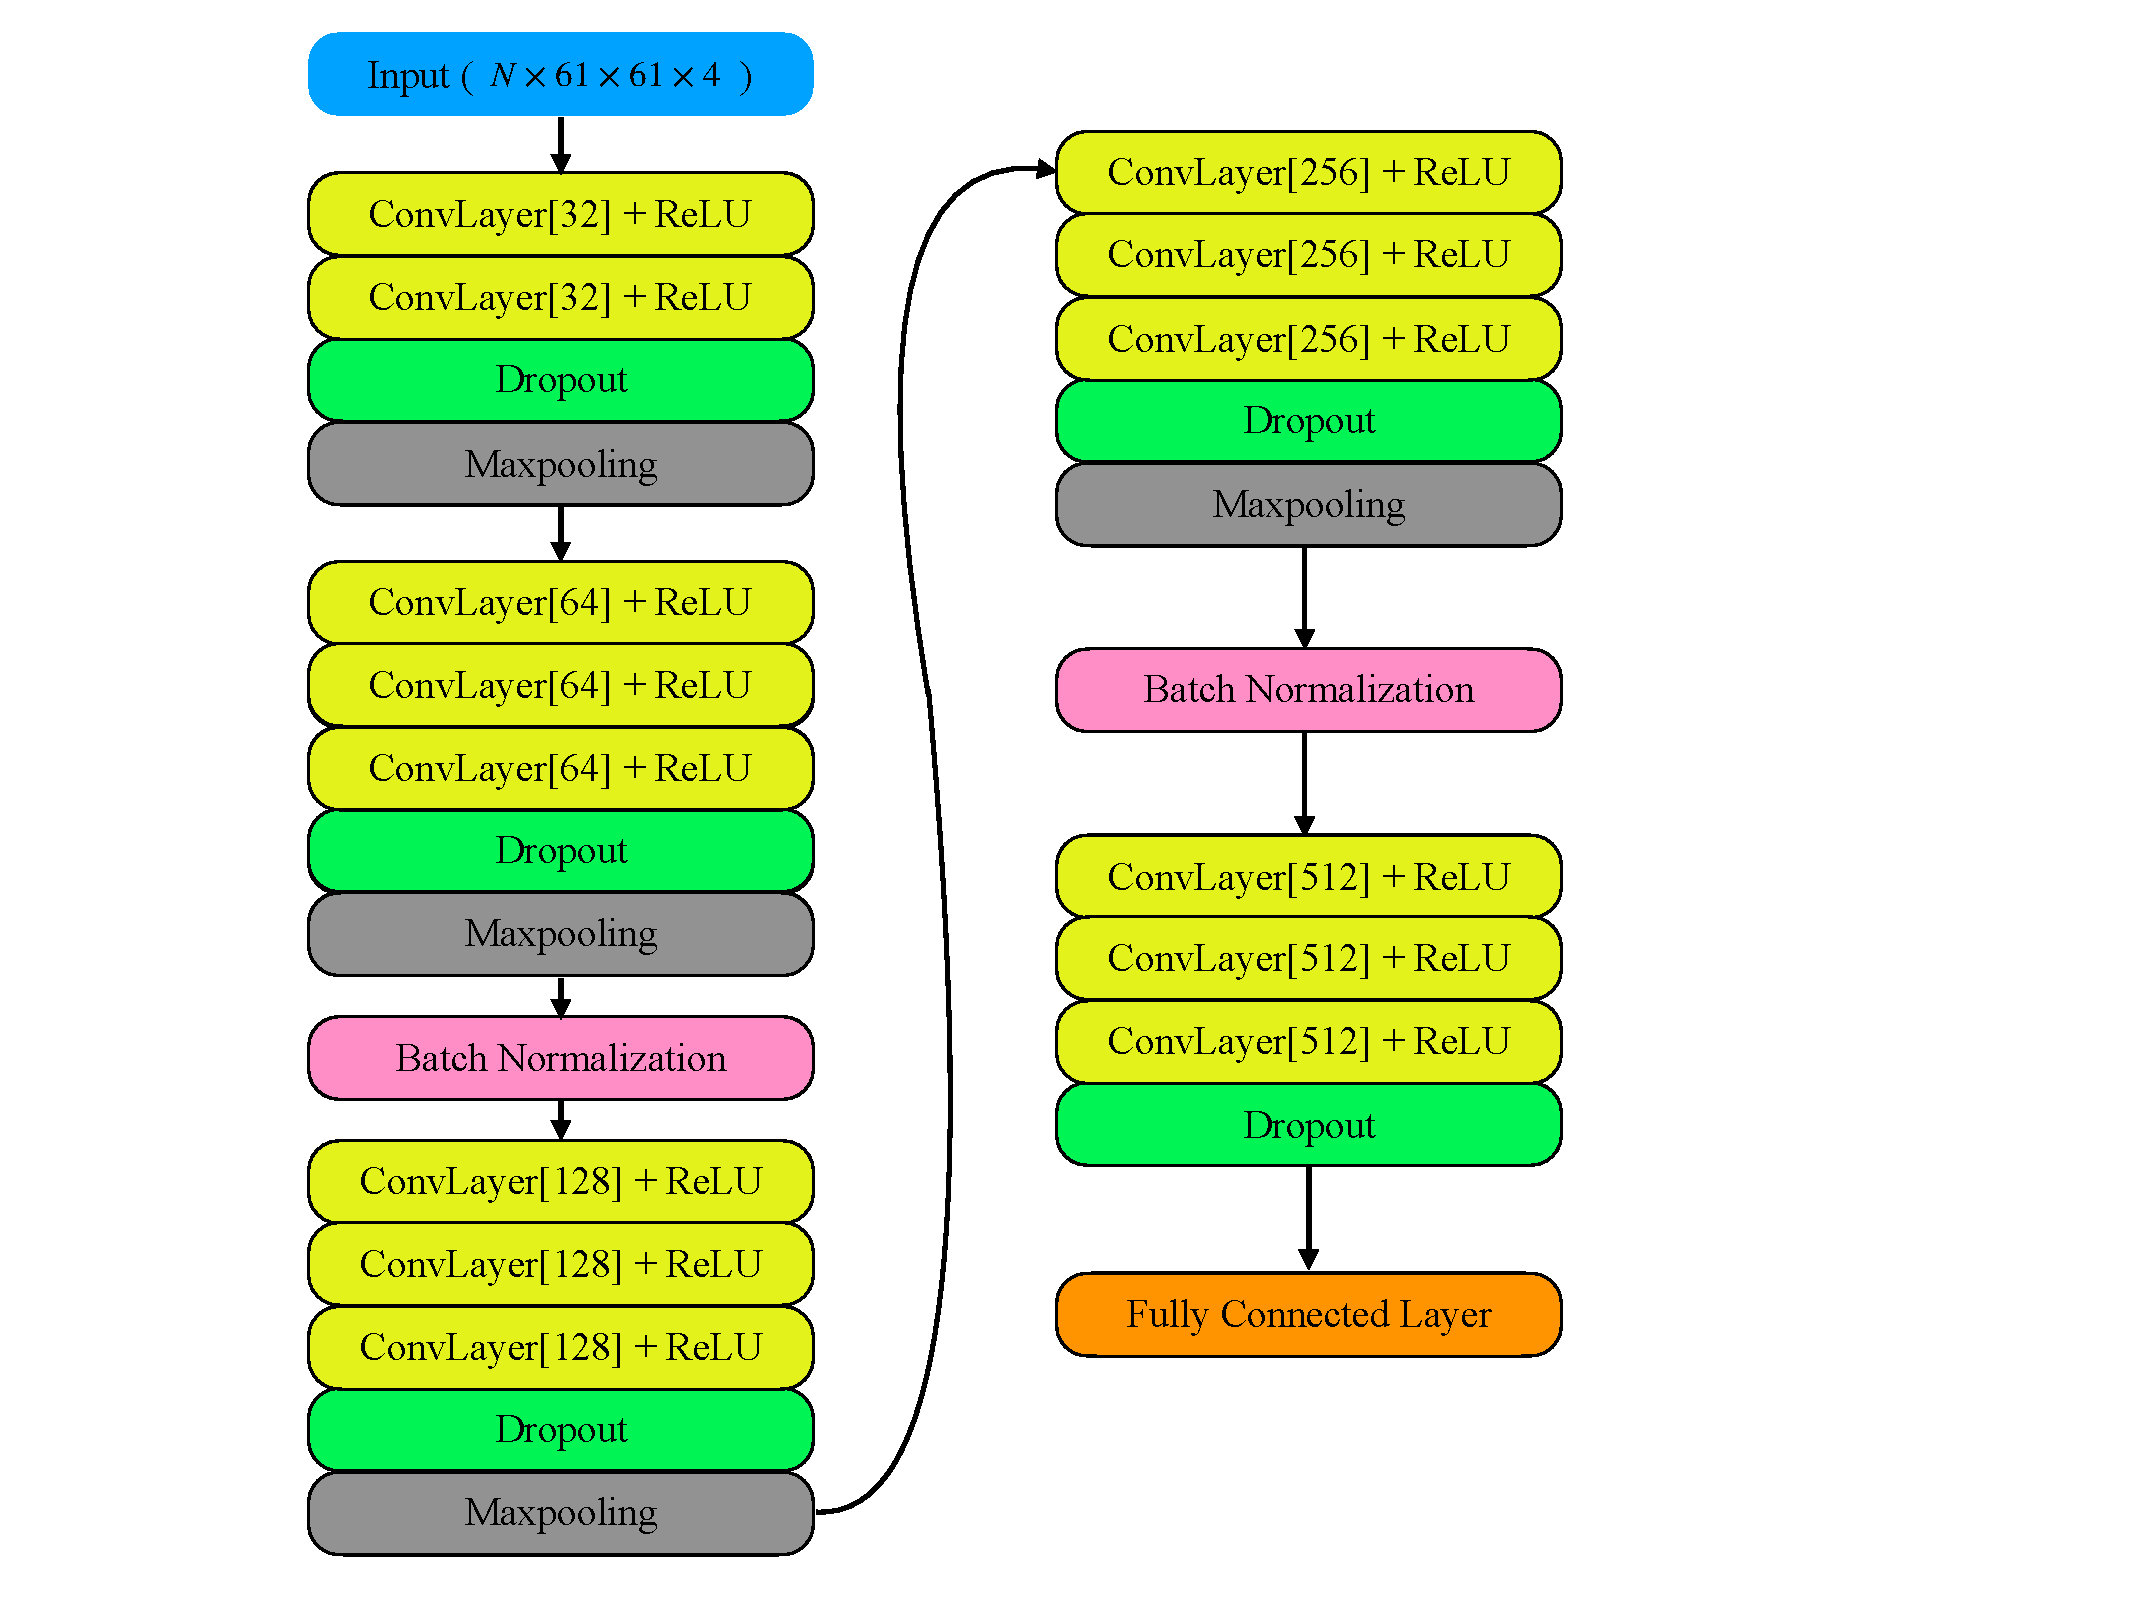
\includegraphics[width=\textwidth]{Figures/cnn_arc.pdf}
        \caption{Architecture of CNN model}
        \label{fig:art}
    \end{figure}

    \begin{table}[h!]
        \centering
        \begin{tabular}{ l | c  }
            Layer & Output Shape  \\ \hline
            Input & $n_b\times61\times61\times4$  \\
            Convolution(32) & $n_b\times61\times61\times32$  \\
            Convolution(32) & $n_b\times61\times61\times32$  \\
            Dropout & $n_b\times61\times61\times32$  \\
            MaxPooling & $n_b\times31\times31\times32$ \\
            Convolution(64) & $n_b\times31\times31\times64$  \\
            Convolution(64) & $n_b\times31\times31\times64$  \\
            Convolution(64) & $n_b\times31\times31\times64$  \\
            Dropout & $n_b\times31\times31\times64$  \\
            MaxPooling & $n_b\times16\times16\times64$ \\
            BatchNormalization & $n_b\times16\times16\times64$ \\
            Convolution(128) & $n_b\times16\times16\times128$  \\
            Convolution(128) & $n_b\times16\times16\times128$  \\
            Convolution(128) & $n_b\times16\times16\times128$  \\
            Dropout & $n_b\times16\times16\times128$  \\
            MaxPooling & $n_b\times8\times8\times128$ \\
            Convolution(256) & $n_b\times8\times8\times256$  \\
            Convolution(256) & $n_b\times8\times8\times256$  \\
            Convolution(256) & $n_b\times8\times8\times256$  \\
            Dropout & $n_b\times8\times8\times256$  \\
            MaxPooling & $n_b\times4\times4\times256$ \\
            BatchNormalization & $n_b\times4\times4\times512$  \\
            Convolution(512) & $n_b\times4\times4\times512$  \\
            Convolution(512) & $n_b\times4\times4\times512$  \\
            Convolution(512) & $n_b\times4\times4\times512$  \\
            Dropout & $n_b\times4\times4\times512$ \\
            Flatten & $n_b\times8192$ \\
            Dense & $n_b\times7442$ \\    
        \end{tabular}
        \caption{Feature map (tensor) sizes through the network, the input has size $n_b\times61\times61\times5$, with batch size $n_b$ and patches of size $61\times61\times5$.}
        \label{table:layers}
    \end{table}

\subsection{Traing Configuration}
\subsubsection{Loss Function}
Firstly, we define a filter funtion,
\begin{equation}
    g(x)= \begin{cases} 0, \quad x = 0 \\ 1, \quad x \ne 0 \end{cases}
\end{equation}
Then, we can update the loss function based on Euqation \ref{eq:mse}. 

\begin{equation}
    L = \frac{1}{N}\sum_{i}^{N}g(\hat{y}_i)(y_i-\hat{y}_i)^2
\end{equation}

\subsection{Training Details}
    The learning happened on GPU(\textit{GeForce GTX 1080 Ti, 11 Gbps GDDR5X memory})\footnote{\url{https://www.nvidia.com/en-us/geforce/products/10series/geforce-gtx-1080-ti/}} held by Image Section, DIKU\footnote{\url{https://di.ku.dk/english/research/imagesection/}}. The whole learning takes nearly 24 hours. The model you can download in my personal dropbox\footnote{\url{https://www.dropbox.com/s/jrwzqib6ghrq59i/model.h5?dl=0}}. I gave hyperparameters setting below,
    \begin{table}[h!]
        \centering
        \begin{tabular}{ l | c  }
            Hyperparameter  & Setting \\ \hline
            Activation function & ReLU \\
            Weight initilization & He normal\cite{sutskever2013importance} \\
            Weight regularizer &  L2 \cite{hinton2006fast} \\
            Convolution border mode  & Same \\
            Stride & 2 \\ 
            Kernel size & $(3, 3)$ \\
            Dropout rate & $0.1$ \\
            Optimizer & SGD \\
            Initial Learning Rate & $1\times 5\times10^{-3}$ \\
            Batch Size & 200 \\
            Epoch & 1000 \\
            Validation Rate & 0.2 \\
        \end{tabular}
        \caption{Hyperparameter settings.}
        \label{table:hyper}
    \end{table}
    \subsubsection{Learning Rate}
    The learning rate will change with the number of epoch, as talked in section \ref{learning}. I will give a specific value as the learning rate depending on the number of epoch. The learning rate will become smaller with increasing epoch. 
    data. The overall algorithm is concluded in Algorithm \ref{ls}.

    \subsubsection{Conclusion about Training process}
    \begin{itemize}
        \item The size of the input image is $41\times41\times4$, and all pixels are important since all of them retore useful information. If we want to extract the features from $41\times 41$, $3\times 3$ kernel would be a good choice. But the disadvantages is that there would be a lot of training parameters, which might slow down the learning process.
        \item I do have nearly $18208$ samples for training. However, it is hard for both the GPU and CPU to load all the data at one time. Dividing all training samples to a couple of batches would not only speed up the single training time and release memory, but also reduce the risk of overfitting.
        \item The learning rate will change with the number of the epoch, as analyzed in section \ref{learning}. I will give a specific learning rate values depending on the number of the epoch. The learning rate will become smaller with With the epoch increase, I hope the value of learning rate can decrease. Since the high learning rate would cause suboptimal performance at the end of training. The overall algorithm is concluded in Algorithm \ref{ls}.
        \item Validation data set is essential to test the accuracy of the model and whether it is overfitting. Before each epoch, validation would be randomly selected, $20\%$ of total data.
    \end{itemize}

    \begin{algorithm}[!h]
        \KwData{$epoch$}
        \KwResult{learning rate $\eta$}
        \If {$epoch < 100$}{$\eta = 5\times10{-3}$}
        \If {$100< epoch < 300$}{$\eta = 2\times10^{-3}$}
        \If {$300< epoch < 500$}{$\eta = 1\times10^{-3}$}
        \If {$epoch > 300$}{$\eta = 2\times10^{-4}$}
        \caption{Learning Rate Scheduling}
        \label{ls}
    \end{algorithm}


\section{Simualtion based on Trained Model}
Once getting the trained model, the next step is to apply this model in simulation based on Algorithm \ref{al:basic} and compare it with other solutions. The details of process is described in Algorithm \ref{al:basic}
\begin{figure}[!h]
    \centering
    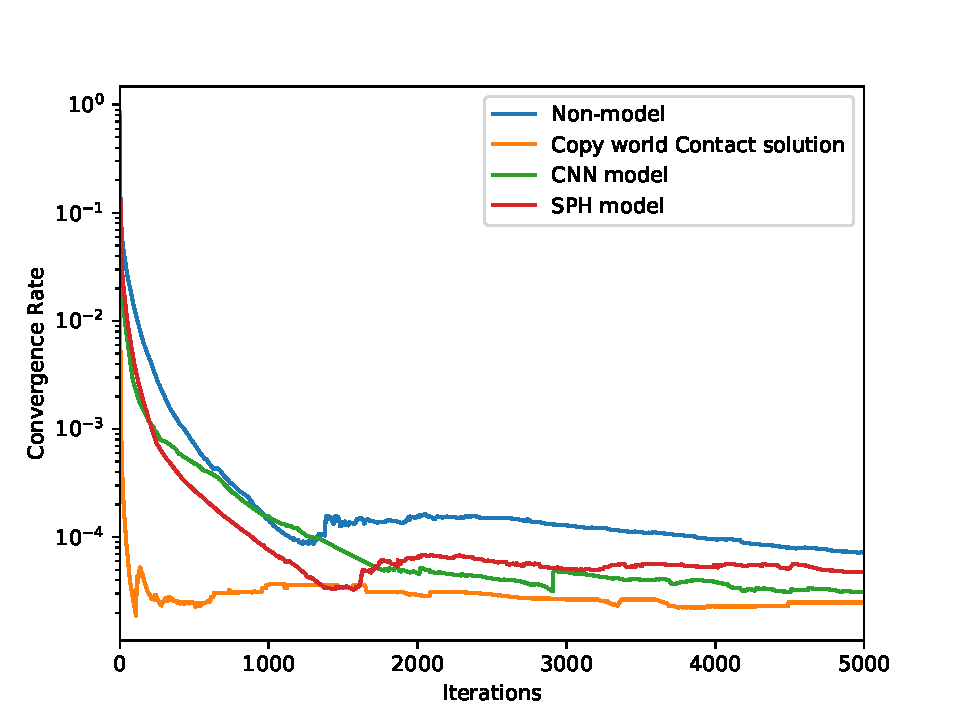
\includegraphics[width=0.8\textwidth]{Figures/same_world.pdf}
    \caption{The final result. Add the final CNN solution to compare with other methods.}
    \label{testoneworld}
\end{figure}

I applied it in one test world built by the setting mentioned in section \ref{simconfig}. The test world is consist one $30 \times 30 $ box and $K$($50<K<100$) randomly distributing balls($r=1$). The balls will fall down due to gravity. Figure \ref{testoneworld} shows the details. As what is expected, CNN model performs similar with \textbf{SPH-Model}(mentioned in section \ref{sphtest}). Although the model is not as good as \textbf{SPH-model}, its coverages rate is obviously faster than built-in ones. 
From Figure \ref{testoneworld}, it can be indicated that the CNN model actually makes the iterative solver converge faster. But it is just a small improvement. The CNN solution cannot reach a convergence as rapidly as \textbf{Copy-Model}. It is mainly the limitation of the SPH-based method. When the particle .

\begin{algorithm}[!h]
        \KwData{
            Given a set of bodies $\mathcal{B}$ and the state in time $t$, as well as some information of contacts between these bodies $\mathcal{C}$.
        }
        \KwResult{Get the contact forces $\pmb{\lambda}_{j}=[{\lambda_{n}}_{j}, {\lambda_{t}}_j]~~j\in\mathcal{C}$ at time $t$.}
        \While{Simulation Runing}
        {
            1. read the current state, $\mathbf{x}=(x_i, y_i)$ is the spatial position of one node in the grid image.
                $$m_i, \pmb{v}_i, \pmb{q}_i, \omega_{i}~~i\in\mathcal{B}$$
                $$\pmb{n}_j~~j\in\mathcal{C}$$ \\
            2. map the current state to a gird image,
                $$G_{m}(\mathbf{x}) \equiv \sum_{i\in \mathcal{B}}W(\mathbf{x}, \pmb{q}_{i})m_i$$ 
                $$G_{\pmb{v}}(\mathbf{x}) \equiv \sum_{i\in \mathcal{B}}W(\mathbf{x}, \pmb{q}_{i})\pmb{v}_i,~~\pmb{v}=(v_x, v_y)$$
                $$G(\mathbf{x}) = [G_{m}(\mathbf{x}), G_{\pmb{v}}(\mathbf{x}), G_{\pmb{n}}(\mathbf{x})]$$ \\
            3. Use $G(\mathbf{x})$ as the input image to the learning model, the output will be resize to a imag, the output image will be called $G_{output}$,
                $$G_{output}(\mathbf{x}) = [G_{\lambda_{n}}(\mathbf{x}), G_{{\lambda}_{t}}(\mathbf{x})]$$ \\
            4. Once the contact force image is obtained,  the conatct position $\pmb{q}_{j} = (x_{j}, y_{j})~~j\in\mathcal{C}$  will be used to interpolation image values based on Equation \ref{interpolation}.
                $$\pmb{\lambda}_j \approx G_{output}(\pmb{q}_j)~~j\in\mathcal{C}$$ 
            The interpolated values $\pmb{\lambda}$ will be used as starting iterated for \textit{pybox2d} conatc solver to find a final solution. \\
            5. Update $t$
                $$t = t + \Delta t$$ \\
        }
        \caption{Introducrion to the deep contact model solver in this thesis.}
        \label{al:basic}
\end{algorithm}

    \chapter{Conclusion and Future Work}

\section{Conclusion}
Half one year ago, I had to formulate a set of goals for the work of this thesis. The goals were thus set before having gained the knowledge I have now. For this reason, the goals reached may appear slightly different from those set. I started out thinking that it would be better to train learning models for normal and friction forces respectively. After four-moonths considering, I have to face the problem that normal force prediction would use the same grid images with friction force. Besdies, the output size of these models would be the same as well. So, training two models equals to training one model with more convolutional layer and extended fully connected layer. 
\begin{itemize}
    \item \textbf{Describe the contact model by \textit{Newton-Euler} equation}, this is described in Chapter \ref{cp:contact}. Normally, the contact model can be derived as a linear complementarity problem formulation(Equation \ref{contactlcp}), which can solved by number.
    \item \textbf{Analyze SPH kernel}, I introduced two smoothing kernel in this project, \textbf{Poly6} and \textbf{Spiky}. Intially, I tried to choose one kernel firstly, and then determine parameters(grid size and smoothing length). However, I found it would be smart to find good grid size($d$) and smoothing length($h$) respectively, then compare the performance of two kernels with good parameters.  
    \item \textbf{Analyze grid size and smoothing length}, the analysis about grid cell size and smoothing length can be found in Figure \ref{poly6} and Figure \ref{spiky}.
    \item \textbf{CNN design}, the CNN architecture can be reviewed in Figure \ref{fig:art}. Since there are no standard for CNN structure designing. I got the inspiration from AlexNet.
    \item \textbf{Comparision among different model solution}, the results describing the difference among \textbf{Copy-Model}, \textbf{SPH-Model}, \textbf{None-Model} and \textbf{CNN-Model}, were shown in Figure \ref{fg:nosph}, Figure \ref{fg:addsph} and Figure \ref{testoneworld}.
    \item \textbf{Training both normal forces and friction forces}, depending on the feature of CNN, training models for normal and friction forces respectively, equals to training one model with more convolutional filters and layers, which can predict both of normal and friction forces.
\end{itemize}

\section{Future Work}
\subsection{SPH-based method}
\begin{itemize}
    \item For the SPH-based method, it is still far away from perfect. It performs not much better than warm starting. So in the future, exploring deeper in SPH-based will help to improve the whole process. The probable attempt will including trying more new kernels, which could stay 
    \item The interpolation used in this project is just one simple linear interpolation. I thought it would lose some essential information when it was interpolated back to particles. So exploring another interpolation method would be helpful to this project.
    \item If we want to use the CNN model to replace built-in warm starting, the biggest issue is simulation time. Although the CNN model can reach convergence more quickly than built-in warm starting method, it cannot replace the built-in method due to long-time spending. It takes a long time to do interpolation. So an efficient and accurate method or data structure for interpolation would speed up the whole process.
\end{itemize}

\subsection{CNN architeture}
Since the peformance of \textbf{CNN-Model} is close to \textbf{SPH-Model}, I think this CNN architecture is a good design and predicts the grid values well. However, in the future, more comlicated CNN structure should be tried on improving the accuracy of prediction.


\subsection{More experiments}
Since current experiments and attempts are all based on same-size circle objects, I hope more experiments can be carried out on circle objects in different size or different shapes(eg. trangle, rectangle).

    \printbibliography[heading=bibintoc, title={References}]
    
    \begin{appendices}
\linespread{1.0}
\renewcommand{\thechapter}{\Alph{chapter}.}
\chapter{Smoothed Particle Hydrodynamics}
\section{Smoothing Kernels}
\begin{python}
def W_poly6_2D(r, h):
    '''
    :param r: A 2d matrix where each column is a vector
    :param h: Support radius
    :return:
    '''
    assert r.shape[0] == 2

    # We determine the length of the vectors and pick out those with length below h
    r_norm = np.linalg.norm(r, axis=0)
    W = np.zeros(r_norm.shape)
    W_i = np.where(r_norm < h)

    # We determine the weights
    c = 4 / (np.pi * np.power(h, 8))
    h2 = np.power(h, 2)
    W[W_i] = c * np.power(h2 - np.power(r_norm[W_i], 2), 3)

    # We normalize the weights so that they add up to 1
    W_sum = np.sum(W)
    W = W / W_sum

    return W

def spiky_2D(r, h):
    assert r.shape[0] == 2

    r_norm = np.linalg.norm(r, axis=0)
    W = np.zeros(r_norm.shape)
    W_i = np.where(r_norm < h)

    c = 15 / (np.pi * np.power(h, 6))
    h2 = np.power(h, 2)
    W[W_i] = c * np.power(h - np.abs(r_norm[W_i]), 3)

    # We normalize the weights so that they add up to 1
    W_sum = np.sum(W)
    W = W / W_sum

    return W
\end{python}

\chapter{Deep Learning}
\section{Loss Function}
\label{lf}
\begin{python}
def loss_func(y_true, y_pred):
    # remove 0 in y_true
    flags = tf.to_float(K.not_equal(y_true, 0.0))
    return K.mean(K.square((y_pred - y_true) * flags), axis=-1)
\end{python}

\section{CNN architecture}
\label{cnnn}
\begin{python}
def build_model(self, input_shape, output_shape):
        self.model.add(
            Conv2D(
                32,
                (3, 3),
                padding='same',
                kernel_regularizer=keras.regularizers.l2(self.weight_decay),
                kernel_initializer='he_normal',
                input_shape=input_shape))
        self.model.add(Activation('relu'))

        self.model.add(
            Conv2D(
                32,
                (3, 3),
                padding='same',
                kernel_regularizer=keras.regularizers.l2(self.weight_decay),
                kernel_initializer='he_normal',
                input_shape=input_shape))
        self.model.add(Activation('relu'))

        self.model.add(MaxPooling2D(pool_size=(2, 2),
                                    strides=(2, 2),
                                    padding='same'))

        self.model.add(
            Conv2D(
                64,
                (3, 3),
                padding='same',
                kernel_regularizer=keras.regularizers.l2(self.weight_decay),
                kernel_initializer='he_normal'))
        self.model.add(Activation('relu'))

        self.model.add(
            Conv2D(
                64,
                (3, 3),
                padding='same',
                kernel_regularizer=keras.regularizers.l2(self.weight_decay),
                kernel_initializer='he_normal'))
        self.model.add(Activation('relu'))

        self.model.add(
            Conv2D(
                64,
                (2, 2),
                padding='same',
                kernel_regularizer=keras.regularizers.l2(self.weight_decay),
                kernel_initializer='he_normal'))
        self.model.add(Activation('relu'))

        self.model.add(MaxPooling2D(pool_size=(2, 2),
                                    strides=(2, 2),
                                    padding='same'))

        self.model.add(BatchNormalization())
        self.model.add(
            Conv2D(
                128,
                (2, 2),
                padding='same',
                kernel_regularizer=keras.regularizers.l2(self.weight_decay),
                kernel_initializer='he_normal'))
        self.model.add(Activation('relu'))

        self.model.add(
            Conv2D(
                128,
                (2, 2),
                padding='same',
                kernel_regularizer=keras.regularizers.l2(self.weight_decay),
                kernel_initializer='he_normal'))
        self.model.add(Activation('relu'))

        self.model.add(
            Conv2D(
                128,
                (2, 2),
                padding='same',
                kernel_regularizer=keras.regularizers.l2(self.weight_decay),
                kernel_initializer='he_normal'))
        self.model.add(Activation('relu'))

        self.model.add(MaxPooling2D(pool_size=(2, 2),
                                    strides=(2, 2),
                                    padding='same'))

        self.model.add(
            Conv2D(
                256,
                (2, 2),
                padding='same',
                kernel_regularizer=keras.regularizers.l2(self.weight_decay),
                kernel_initializer='he_normal'))
        self.model.add(Activation('relu'))

        self.model.add(
            Conv2D(
                256,
                (2, 2),
                padding='same',
                kernel_regularizer=keras.regularizers.l2(self.weight_decay),
                kernel_initializer='he_normal'))
        self.model.add(Activation('relu'))

        self.model.add(
            Conv2D(
                256,
                (2, 2),
                padding='same',
                kernel_regularizer=keras.regularizers.l2(self.weight_decay),
                kernel_initializer='he_normal'))
        self.model.add(Activation('relu'))

        self.model.add(MaxPooling2D(pool_size=(2, 2),
                                    strides=(2, 2),
                                    padding='same'))

        self.model.add(BatchNormalization())
        self.model.add(
            Conv2D(
                512,
                (2, 2),
                padding='same',
                kernel_regularizer=keras.regularizers.l2(self.weight_decay),
                kernel_initializer='he_normal'))
        self.model.add(Activation('relu'))
        self.model.add(
            Conv2D(
                512,
                (2, 2),
                padding='same',
                kernel_regularizer=keras.regularizers.l2(self.weight_decay),
                kernel_initializer='he_normal'))
        self.model.add(Activation('relu'))
        self.model.add(
            Conv2D(
                512,
                (2, 2),
                padding='same',
                kernel_regularizer=keras.regularizers.l2(self.weight_decay),
                kernel_initializer='he_normal'))
        self.model.add(Activation('relu'))

        self.model.add(Dropout(self.dropout))
        self.model.add(Flatten())
        
        output_size = output_shape[0]

        self.model.add(Dense(output_size))
        self.model.add(Activation('relu'))
\end{python}

\section{Learning Rate Scheduler}
\label{lr}
\begin{python}
def scheduler(epoch):
    if epoch <= 100:
        return 0.05
    if epoch <= 400:
        return 0.02
    return 0.01
\end{python}
    
\end{appendices}

\end{document}
